\documentclass[10pt]{article}
\usepackage[letterpaper,margin=0.6in]{geometry}
\usepackage[T1]{fontenc}\usepackage{lmodern}
\usepackage{pdfpages,booktabs,array,longtable}
\usepackage[table]{xcolor}
\usepackage[hidelinks]{hyperref}
\pagestyle{plain}
\renewcommand{\arraystretch}{1.25}
\begin{document}
{\sffamily\bfseries\LARGE Agent-swarm physics: hypothesis compendium}\par\vspace{4pt}
{\small Living status document, regenerated 2026-10-03 17:32 by \texttt{infra/summaries/build\_summaries.py}. Not the paper. One page per hypothesis follows; click a row to jump to it.}\par\vspace{6pt}
{\footnotesize\textbf{Completion}: estimated progress of the research direction (idea 5\%, round 1 done 35--50\%, holdout run 55--65\%, robustness and causal designs 70--85\%, settled 90--100\%). \colorbox[HTML]{cde2fb}{\textcolor[HTML]{0b0b0b}{\scriptsize 5\%}} \colorbox[HTML]{9ec5f4}{\textcolor[HTML]{0b0b0b}{\scriptsize 25\%}} \colorbox[HTML]{5598e7}{\textcolor[HTML]{0b0b0b}{\scriptsize 50\%}} \colorbox[HTML]{256abf}{\textcolor[HTML]{ffffff}{\scriptsize 75\%}} \colorbox[HTML]{184f95}{\textcolor[HTML]{ffffff}{\scriptsize 100\%}}\par
\textbf{Faithfulness} (0--5, scoped): how well the model holds for what it claims (3 = descriptive or primary holdout passed; 4 = supported; 5 = faithful and mechanistic).
\textbf{Usefulness} (0--5, unscoped): what an operator or alignment researcher can do with it, true or not (1 = vocabulary only; 2 = a diagnostic; 3 = a validated monitor or design rule; 4 = a steering lever; 5 = a transferable control knob). \colorbox[HTML]{a32b2b}{\textcolor[HTML]{ffffff}{\scriptsize 0}} \colorbox[HTML]{e34948}{\textcolor[HTML]{0b0b0b}{\scriptsize 1}} \colorbox[HTML]{f5bcbb}{\textcolor[HTML]{0b0b0b}{\scriptsize 2}} \colorbox[HTML]{e9e7e1}{\textcolor[HTML]{0b0b0b}{\scriptsize 2.5}} \colorbox[HTML]{b7d3f6}{\textcolor[HTML]{0b0b0b}{\scriptsize 3}} \colorbox[HTML]{5598e7}{\textcolor[HTML]{ffffff}{\scriptsize 4}} \colorbox[HTML]{1c5cab}{\textcolor[HTML]{ffffff}{\scriptsize 5}}\par
Ratings are estimates calibrated across hypotheses by the coordinator; rubric in \texttt{writeup/hypothesis-pages/RUBRIC.md}.}
\par\vspace{6pt}
\begin{longtable}{@{}p{0.05\textwidth}p{0.6\textwidth}>{\centering\arraybackslash}p{0.075\textwidth}>{\centering\arraybackslash}p{0.075\textwidth}>{\centering\arraybackslash}p{0.075\textwidth}>{\raggedleft\arraybackslash}p{0.04\textwidth}@{}}
\toprule
\textbf{ID} & \textbf{Hypothesis} & \textbf{Complete} & \textbf{Faithful} & \textbf{Useful} & \textbf{p.}\\\midrule\endhead
\hyperlink{H01.1}{\textbf{H01}} & \hyperlink{H01.1}{Emergent superagents exist} \textcolor{gray}{\scriptsize(draft)}\newline{\scriptsize\color{gray}running. Exploratory round 1 of D3.1.a and D3.2 done (2026-10-03, non-holdout only): rooms are reliably more ordered ...} & \textcolor{gray}{--} & \textcolor{gray}{--} & \textcolor{gray}{--} & 3 \\
\hyperlink{H02.1}{\textbf{H02}} & \hyperlink{H02.1}{Inferred couplings reflect real influence} \textcolor{gray}{\scriptsize(draft)}\newline{\scriptsize\color{gray}\#45 confirmation FAILED (locked holdout, run 2026-10-03): the Fine-Tuned Leader ranks 4th of 18 by net outgoing influ...} & \textcolor{gray}{--} & \textcolor{gray}{--} & \textcolor{gray}{--} & 4 \\
\hyperlink{H03.1}{\textbf{H03}} & \hyperlink{H03.1}{Swarm activity is self-exciting, and its criticality is set by the ...} \textcolor{gray}{\scriptsize(draft)}\newline{\scriptsize\color{gray}running. Exploratory round 1 is complete (2026-10-03, non-holdout data only).} & \textcolor{gray}{--} & \textcolor{gray}{--} & \textcolor{gray}{--} & 5 \\
\hyperlink{H04.1}{\textbf{H04}} & \hyperlink{H04.1}{External forcing reshapes the response kernel, reversibly} \textcolor{gray}{\scriptsize(draft)}\newline{\scriptsize\color{gray}confirmatory run on the locked holdout (2026-10-03): C1 FALSIFIED, in the opposite direction. The branching ratio n i...} & \textcolor{gray}{--} & \textcolor{gray}{--} & \textcolor{gray}{--} & 6 \\
\hyperlink{H05.1}{\textbf{H05}} & \hyperlink{H05.1}{Cutting the cross-room channel lowers entropy production, and rooms...} \textcolor{gray}{\scriptsize(draft)}\newline{\scriptsize\color{gray}confirmatory run on the locked holdout (2026-10-03): INCONCLUSIVE by the pre-registered rule. The primary pair DiD at...} & \textcolor{gray}{--} & \textcolor{gray}{--} & \textcolor{gray}{--} & 7 \\
\hyperlink{H07.1}{\textbf{H07}} & \hyperlink{H07.1}{The RPG forks diverge from a common ancestor at a measurable rate} \textcolor{gray}{\scriptsize(draft)}\newline{\scriptsize\color{gray}running. Results are organized by goal period (see "Results by goal period"). Exploratory round 1 (non-holdout: \#35 o...} & \textcolor{gray}{--} & \textcolor{gray}{--} & \textcolor{gray}{--} & 8 \\
\hyperlink{H08.1}{\textbf{H08}} & \hyperlink{H08.1}{Context is the coupling} \textcolor{gray}{\scriptsize(draft)}\newline{\scriptsize\color{gray}idea, parked. Opened 2026-10-03 on a misread: the request was about the thermodynamics framing, which is H09. Kept be...} & \textcolor{gray}{--} & \textcolor{gray}{--} & \textcolor{gray}{--} & 9 \\
\hyperlink{H09.1}{\textbf{H09}} & \hyperlink{H09.1}{Agent swarms have an effective thermodynamics} \textcolor{gray}{\scriptsize(draft)}\newline{\scriptsize\color{gray}exploratory rounds 1 (E1–E5) and 2 (E6–E8) done, light. Observable tables built (idle\_runs, consolidation\_inflow). No...} & \textcolor{gray}{--} & \textcolor{gray}{--} & \textcolor{gray}{--} & 10 \\
\hyperlink{H10.1}{\textbf{H10}} & \hyperlink{H10.1}{Goals are Legendre pushes: a swarm's response to an assigned goal i...} \textcolor{gray}{\scriptsize(draft)}\newline{\scriptsize\color{gray}running (exploratory round 1). Predictions written 2026-10-03 before any real-data run (below).} & \textcolor{gray}{--} & \textcolor{gray}{--} & \textcolor{gray}{--} & 11 \\
\hyperlink{H11.1}{\textbf{H11}} & \hyperlink{H11.1}{Division of labor vs herding is the sign of a Potts coupling, set b...} \textcolor{gray}{\scriptsize(draft)}\newline{\scriptsize\color{gray}exploratory round 1 done (2026-10-03). The sign-by-goal-mode prediction is not supported. $\beta$J\_CW > 0 (herding) in 11 o...} & \textcolor{gray}{--} & \textcolor{gray}{--} & \textcolor{gray}{--} & 12 \\
\hyperlink{H12.1}{\textbf{H12}} & \hyperlink{H12.1}{Groupthink is dimensional collapse: few collective modes, shrinking...} \textcolor{gray}{\scriptsize(draft)}\newline{\scriptsize\color{gray}running. Exploratory round 1 done 2026-10-03: HH77 partially supported (one Curie–Weiss-like market mode, partly join...} & \textcolor{gray}{--} & \textcolor{gray}{--} & \textcolor{gray}{--} & 13 \\
\hyperlink{H13.1}{\textbf{H13}} & \hyperlink{H13.1}{Model families carry their own fields, and couple by family} \textcolor{gray}{\scriptsize(draft)}\newline{\scriptsize\color{gray}exploratory round 1 done (2026-10-04).} & \textcolor{gray}{--} & \textcolor{gray}{--} & \textcolor{gray}{--} & 14 \\
\hyperlink{H14.1}{\textbf{H14}} & \hyperlink{H14.1}{Entropy production of behavior-state sequences: per-family arrows o...} \textcolor{gray}{\scriptsize(draft)}\newline{\scriptsize\color{gray}specified (promoted 2026-10-03 by Vivian from shortlist 2). Exploratory round 1 running: observables, nulls and predi...} & \textcolor{gray}{--} & \textcolor{gray}{--} & \textcolor{gray}{--} & 15 \\
\hyperlink{H15.1}{\textbf{H15}} & \hyperlink{H15.1}{Semantic information through natural scrambles: which information k...} \textcolor{gray}{\scriptsize(draft)}\newline{\scriptsize\color{gray}exploratory round 1 done (2026-10-03, non-holdout only). The pre-registered "memory is load-bearing" predictions fail...} & \textcolor{gray}{--} & \textcolor{gray}{--} & \textcolor{gray}{--} & 16 \\
\hyperlink{H16.1}{\textbf{H16}} & \hyperlink{H16.1}{Agents get stuck in metastable traps and escape by Kramers kinetics...} \textcolor{gray}{\scriptsize(draft)}\newline{\scriptsize\color{gray}specified (promoted 2026-10-03 by Vivian from shortlist 2). Exploratory round 1: synthetic validation done; predictio...} & \textcolor{gray}{--} & \textcolor{gray}{--} & \textcolor{gray}{--} & 17 \\
\hyperlink{H17.1}{\textbf{H17}} & \hyperlink{H17.1}{Behavior is a Markov state model with a few metastable sets; its mi...} \textcolor{gray}{\scriptsize(draft)}\newline{\scriptsize\color{gray}specified (promoted 2026-10-03 by Vivian from HH97). Exploratory round 1 running: observables, nulls and predictions ...} & \textcolor{gray}{--} & \textcolor{gray}{--} & \textcolor{gray}{--} & 18 \\
\hyperlink{H18.1}{\textbf{H18}} & \hyperlink{H18.1}{Attention dilutes as 1/k: response to a message falls with the numb...} \textcolor{gray}{\scriptsize(draft)}\newline{\scriptsize\color{gray}specified (promoted 2026-10-03 by Vivian from HH99). Exploratory round 1: observables, nulls and predictions written ...} & \textcolor{gray}{--} & \textcolor{gray}{--} & \textcolor{gray}{--} & 19 \\
\hyperlink{H19.1}{\textbf{H19}} & \hyperlink{H19.1}{One curve for all periods: per-period loop gains collapse onto a fu...} \textcolor{gray}{\scriptsize(draft)}\newline{\scriptsize\color{gray}running. Exploratory round 1 done (2026-10-04): the pre-registered collapse P1 FAILED, with no common curve: equal-ti...} & \textcolor{gray}{--} & \textcolor{gray}{--} & \textcolor{gray}{--} & 20 \\
\hyperlink{H20.1}{\textbf{H20}} & \hyperlink{H20.1}{Aging: day-to-day content autocorrelation depends on time since kic...} \textcolor{gray}{\scriptsize(draft)}\newline{\scriptsize\color{gray}running (exploratory round 1). Observables, null and predictions written 2026-10-03, before any real-data run (below).} & \textcolor{gray}{--} & \textcolor{gray}{--} & \textcolor{gray}{--} & 21 \\
\hyperlink{H21.1}{\textbf{H21}} & \hyperlink{H21.1}{The debate week (\#12) is a two-sublattice antiferromagnet} \textcolor{gray}{\scriptsize(draft)}\newline{\scriptsize\color{gray}running (exploratory round 1, 2026-10-03). Promoted 2026-10-03 by Vivian from HH103.} & \textcolor{gray}{--} & \textcolor{gray}{--} & \textcolor{gray}{--} & 22 \\
\hyperlink{H22.1}{\textbf{H22}} & \hyperlink{H22.1}{Private, conflicting goals make \#51 a spin glass} \textcolor{gray}{\scriptsize(draft)}\newline{\scriptsize\color{gray}exploratory round 1. Observables, nulls and predictions written 2026-10-04 00:15 UTC (2026-10-03 PT), before any real...} & \textcolor{gray}{--} & \textcolor{gray}{--} & \textcolor{gray}{--} & 23 \\
\hyperlink{H23.1}{\textbf{H23}} & \hyperlink{H23.1}{Distilling the village into a fine-tuned leader copies its vocabula...} \textcolor{gray}{\scriptsize(draft)}\newline{\scriptsize\color{gray}exploratory round 1 running (2026-10-03). Pipeline reconstructed; observables, null and prediction written below befo...} & \textcolor{gray}{--} & \textcolor{gray}{--} & \textcolor{gray}{--} & 24 \\
\hyperlink{H24.1}{\textbf{H24}} & \hyperlink{H24.1}{In the forecast week (\#21), switching from independent drafts to co...} \textcolor{gray}{\scriptsize(draft)}\newline{\scriptsize\color{gray}running (exploratory round 1). Switch-on time determined from the record and predictions written 2026-10-03, before a...} & \textcolor{gray}{--} & \textcolor{gray}{--} & \textcolor{gray}{--} & 25 \\
\bottomrule
\end{longtable}
\clearpage
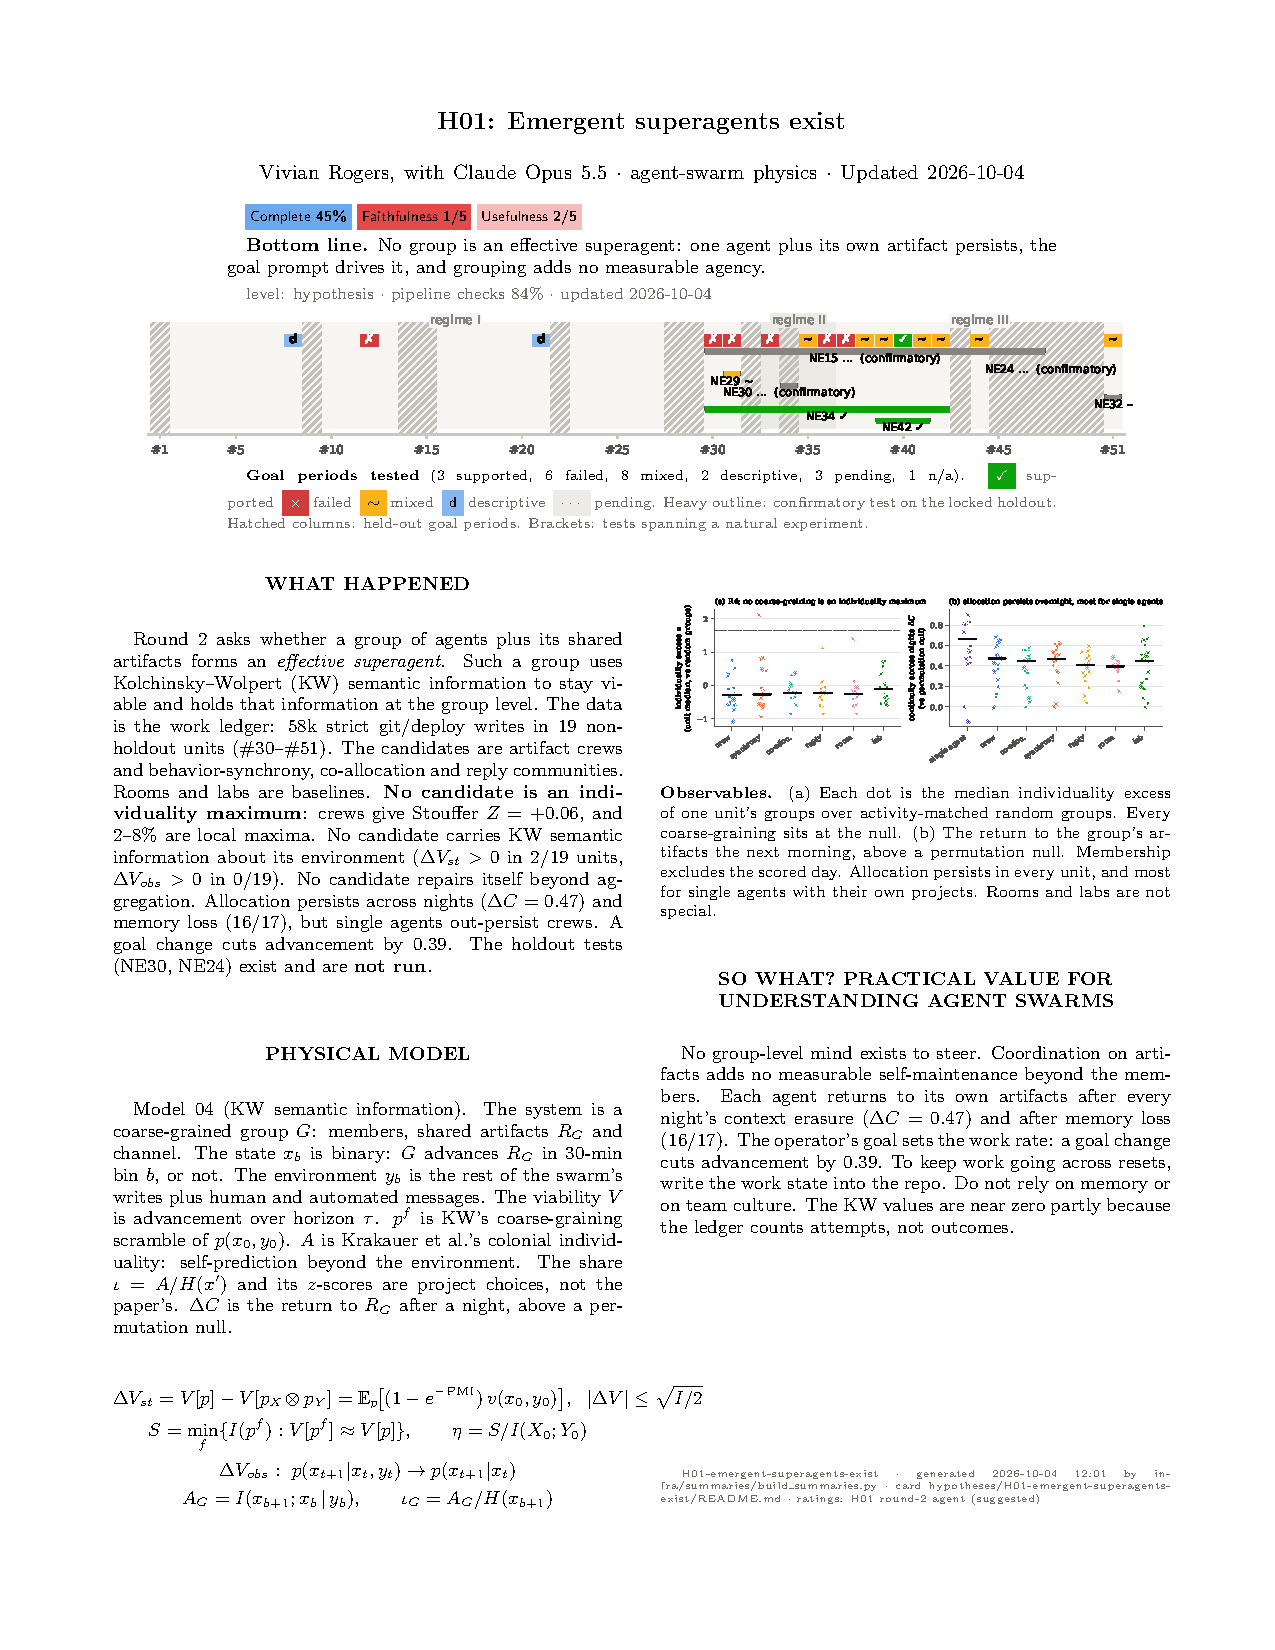
\includepdf[pages=1,link,linkname=H01]{../../hypotheses/H01-emergent-superagents-exist/summary/summary.pdf}
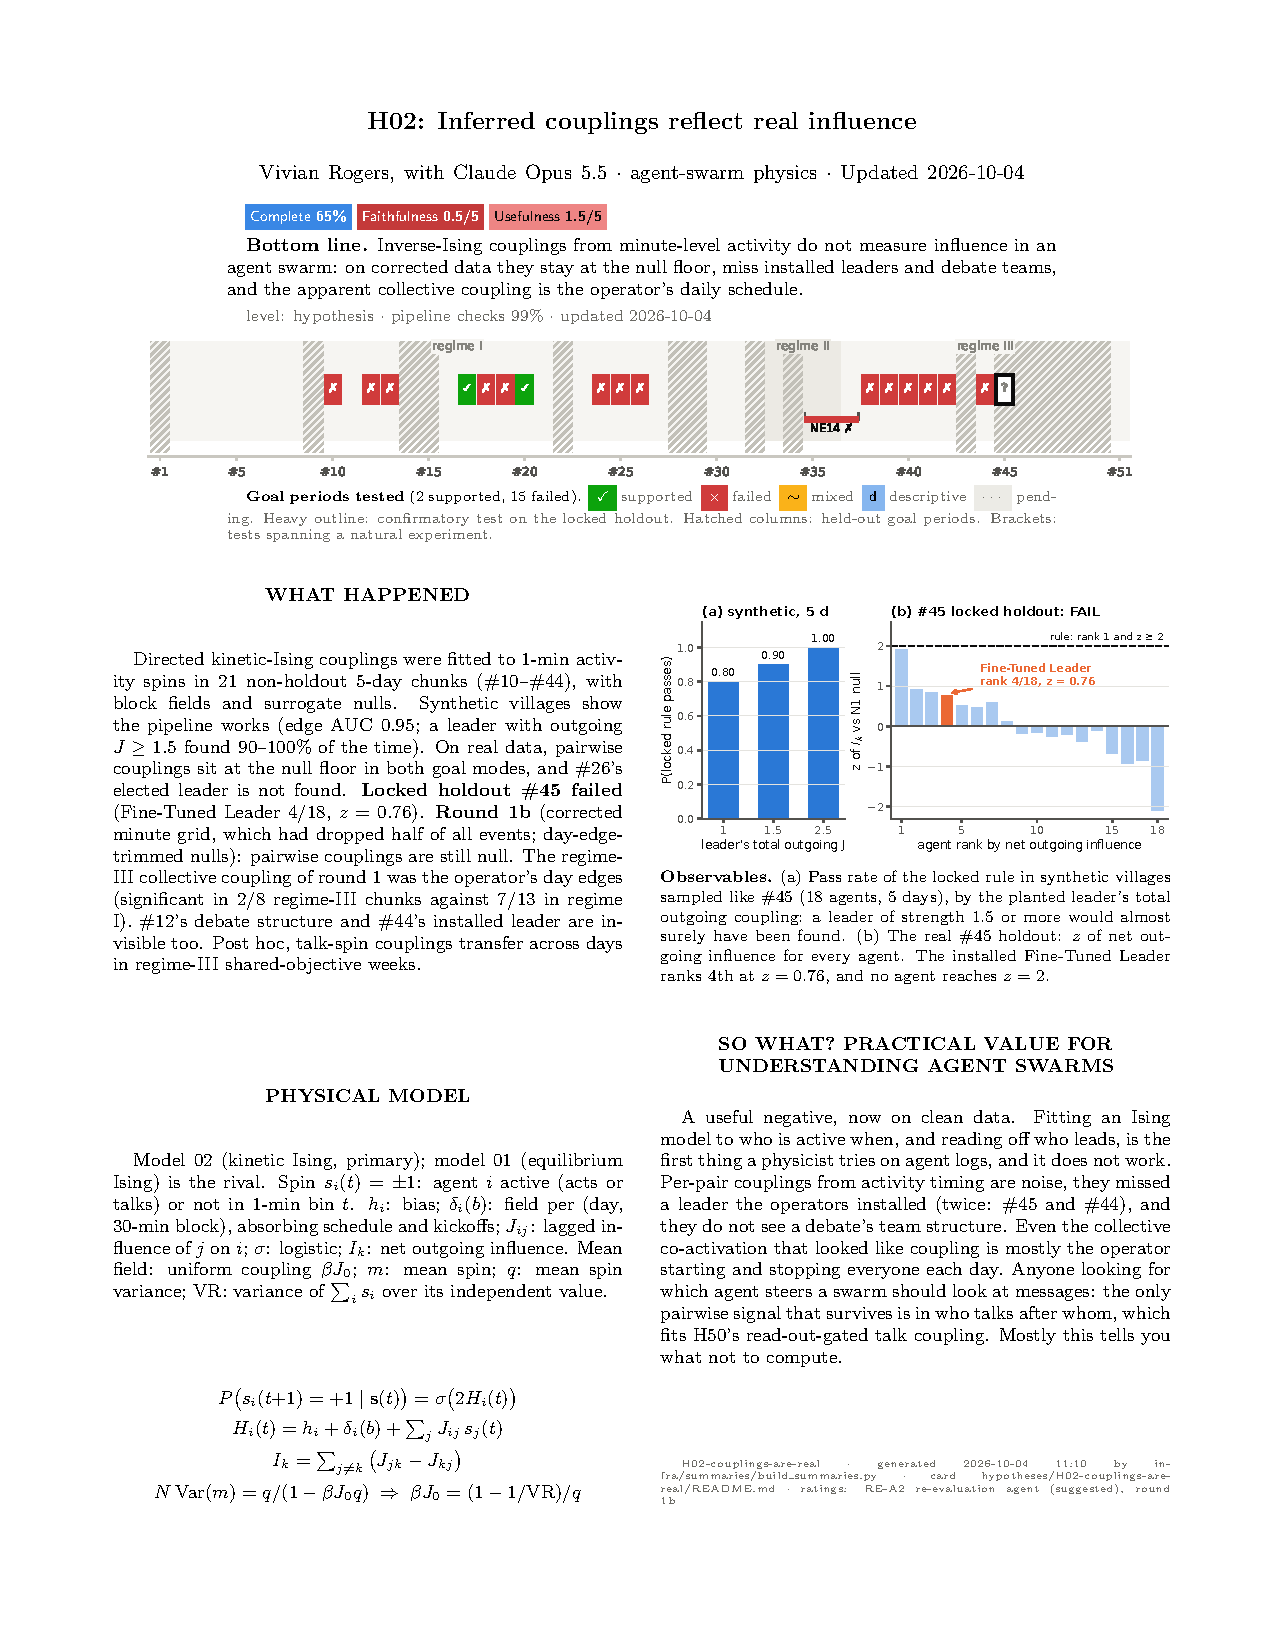
\includepdf[pages=1,link,linkname=H02]{../../hypotheses/H02-couplings-are-real/summary/summary.pdf}
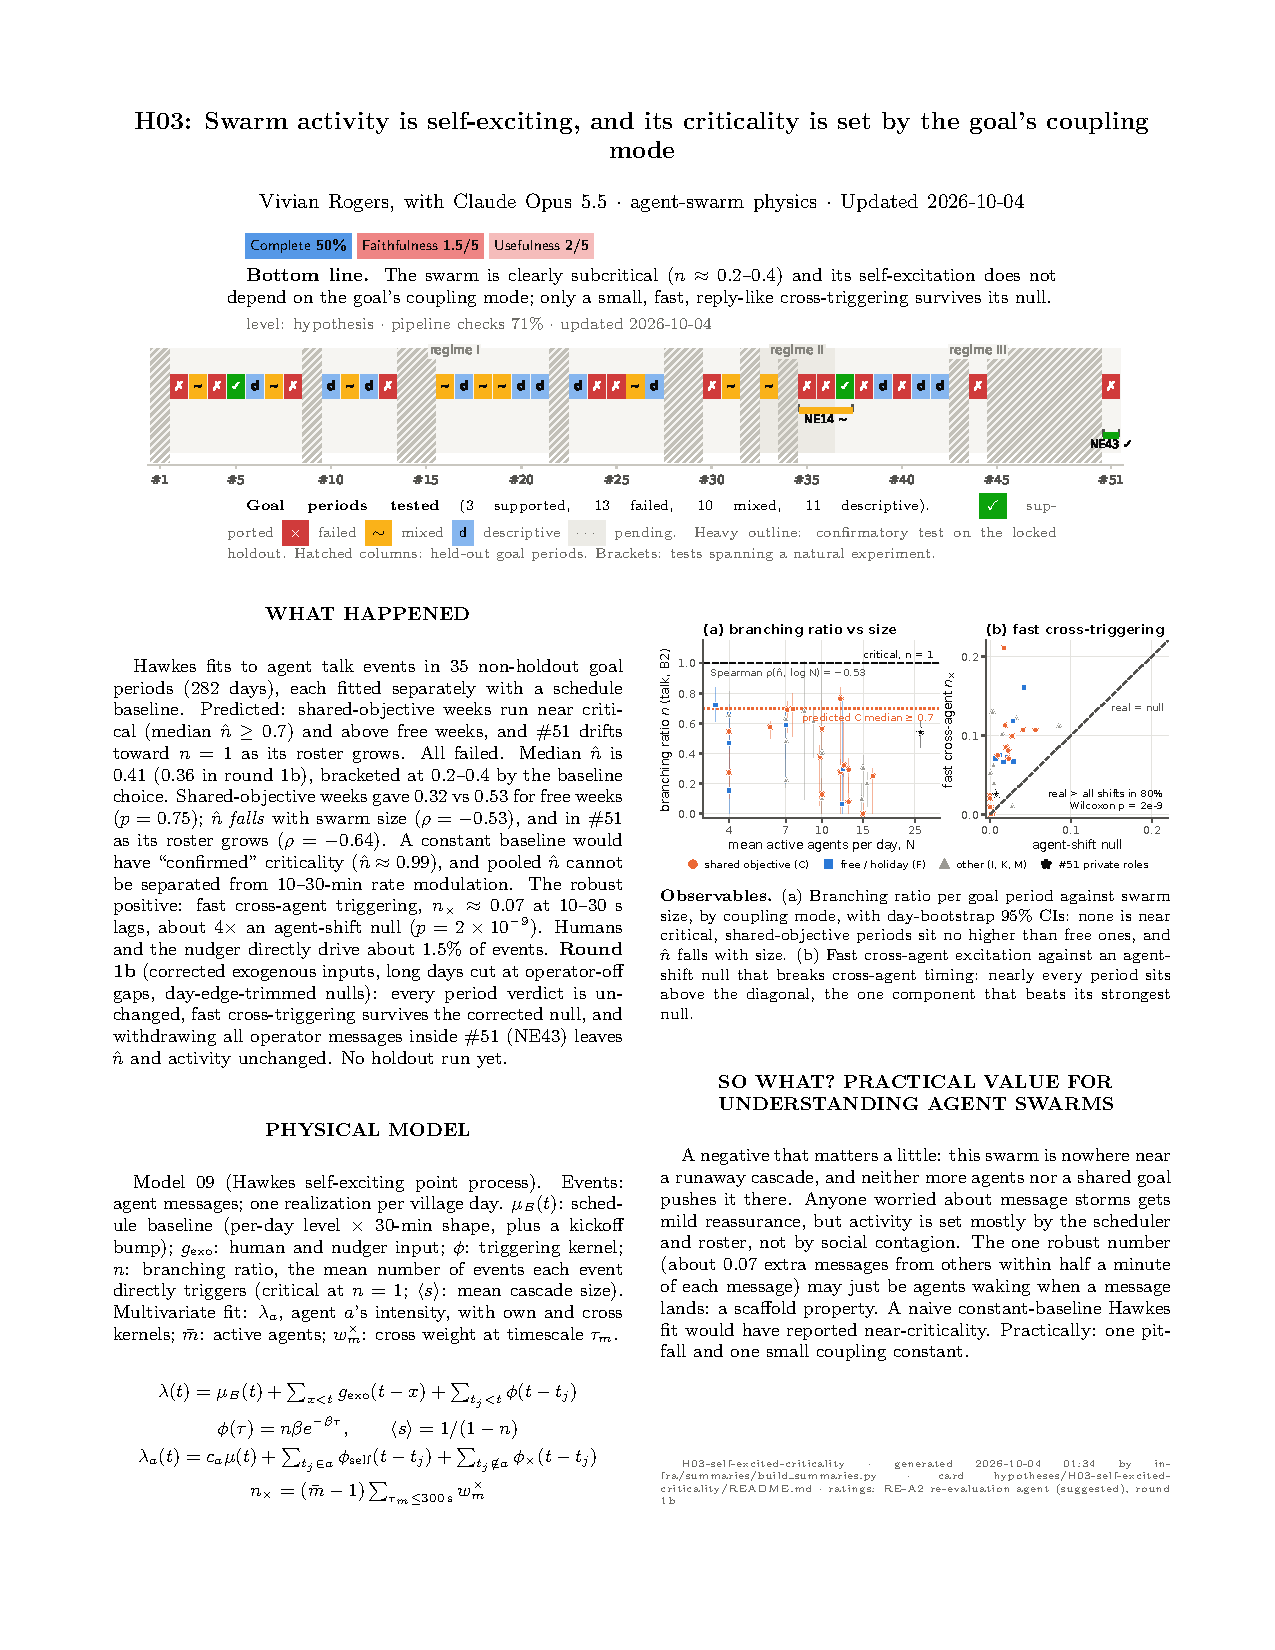
\includepdf[pages=1,link,linkname=H03]{../../hypotheses/H03-self-excited-criticality/summary/summary.pdf}
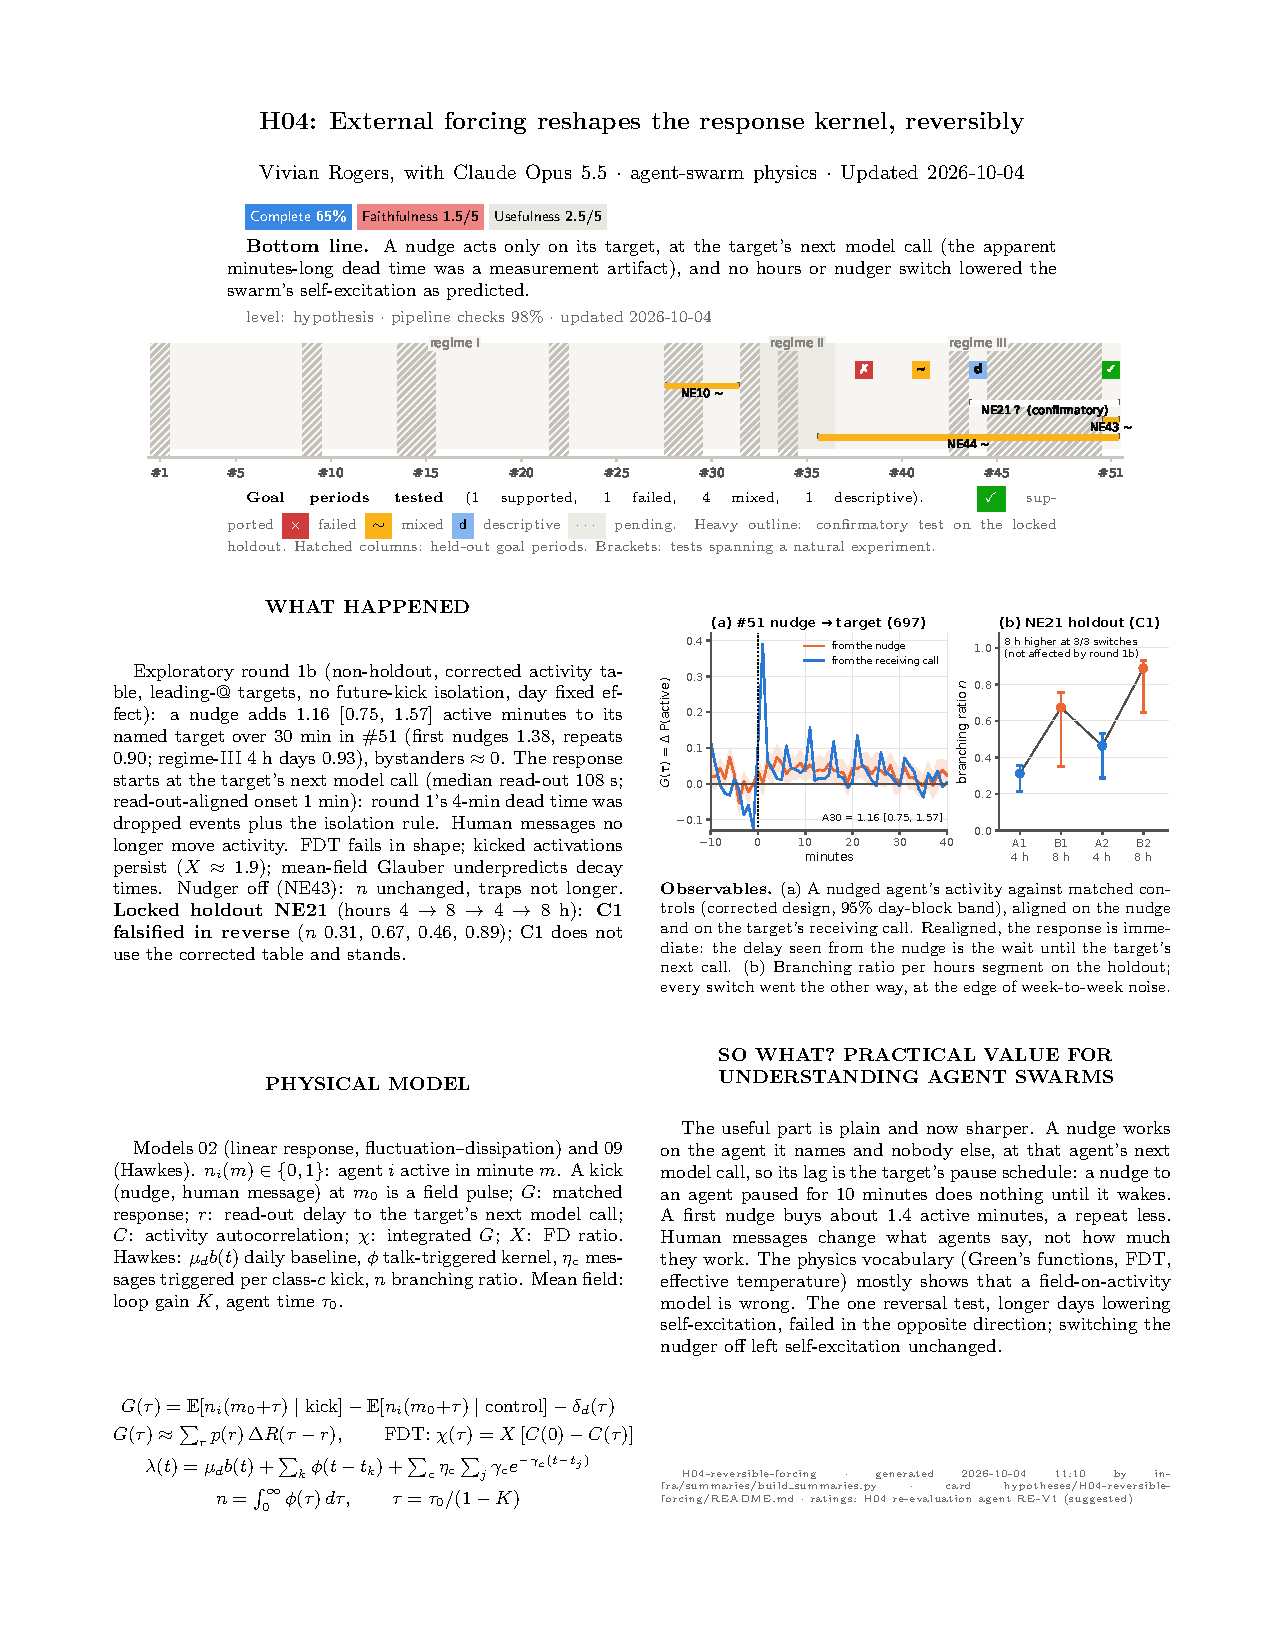
\includepdf[pages=1,link,linkname=H04]{../../hypotheses/H04-reversible-forcing/summary/summary.pdf}
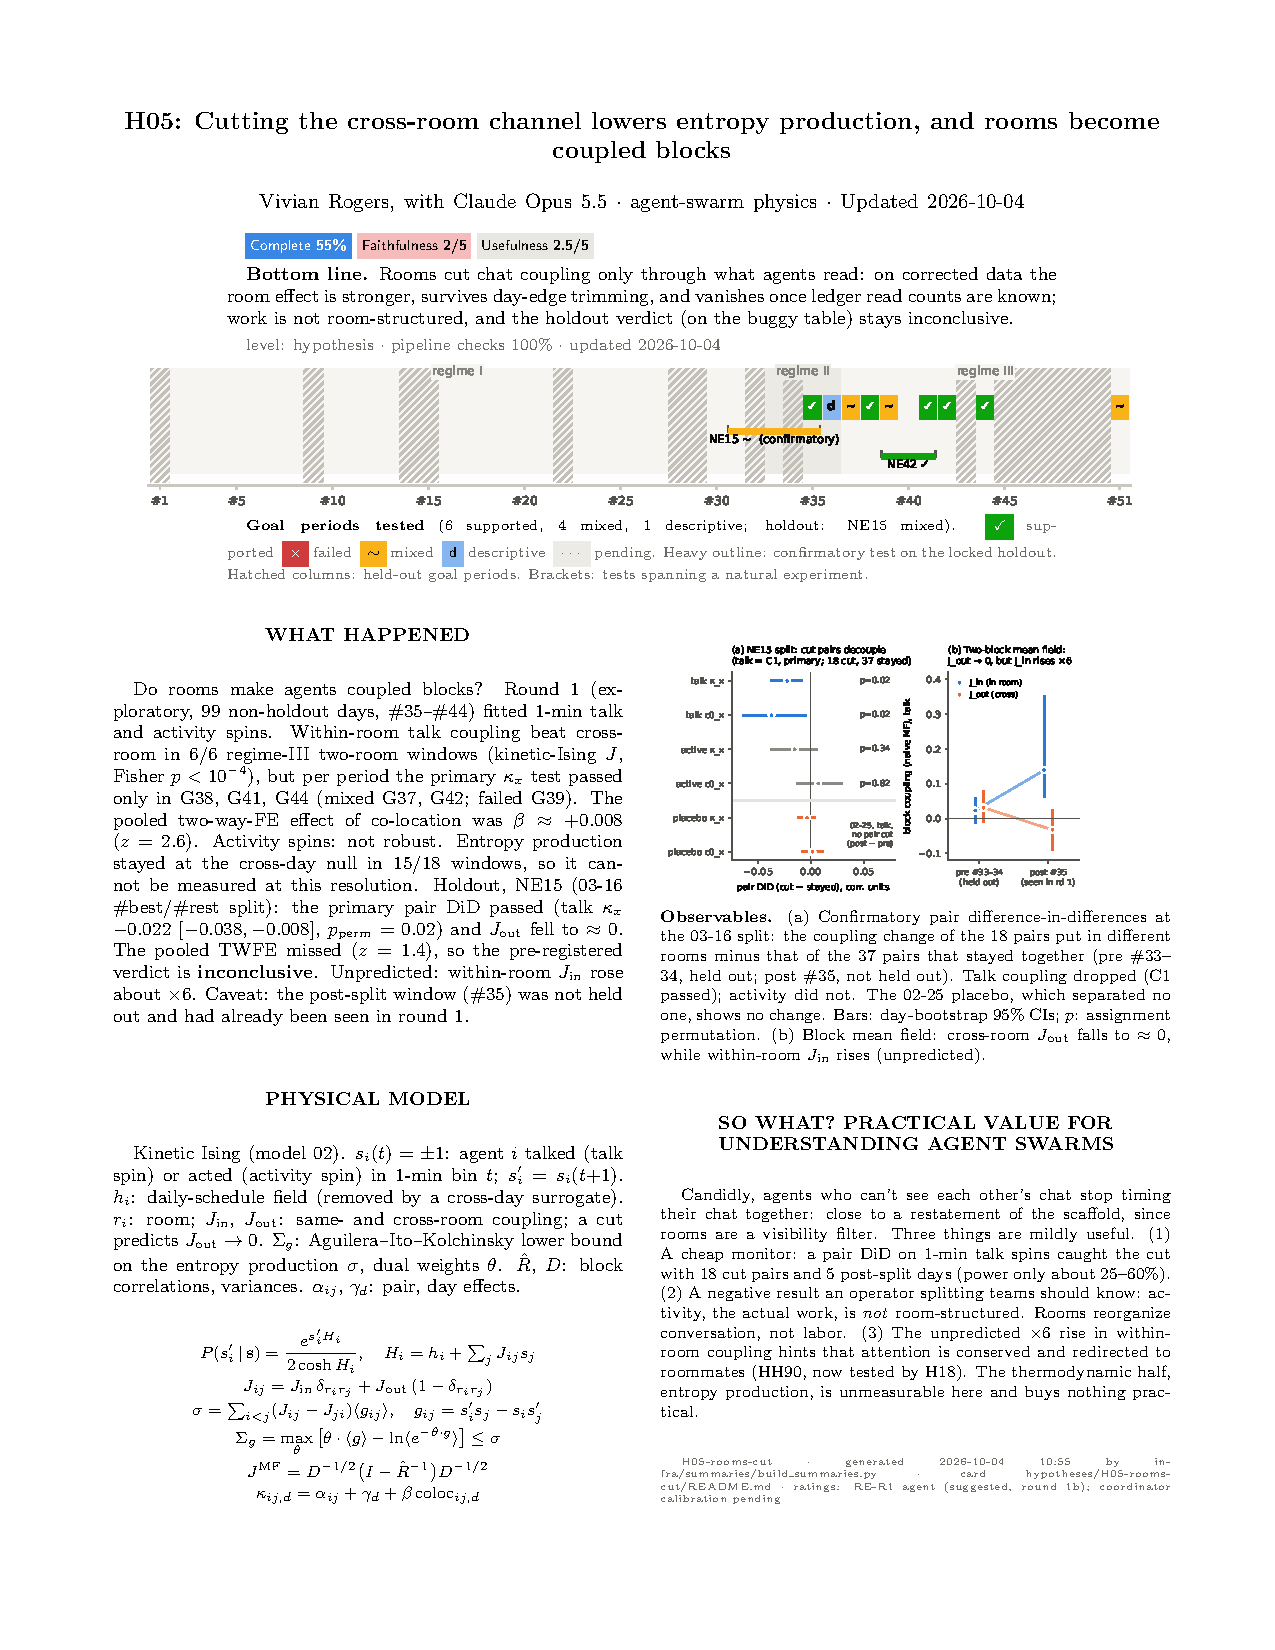
\includepdf[pages=1,link,linkname=H05]{../../hypotheses/H05-rooms-cut/summary/summary.pdf}
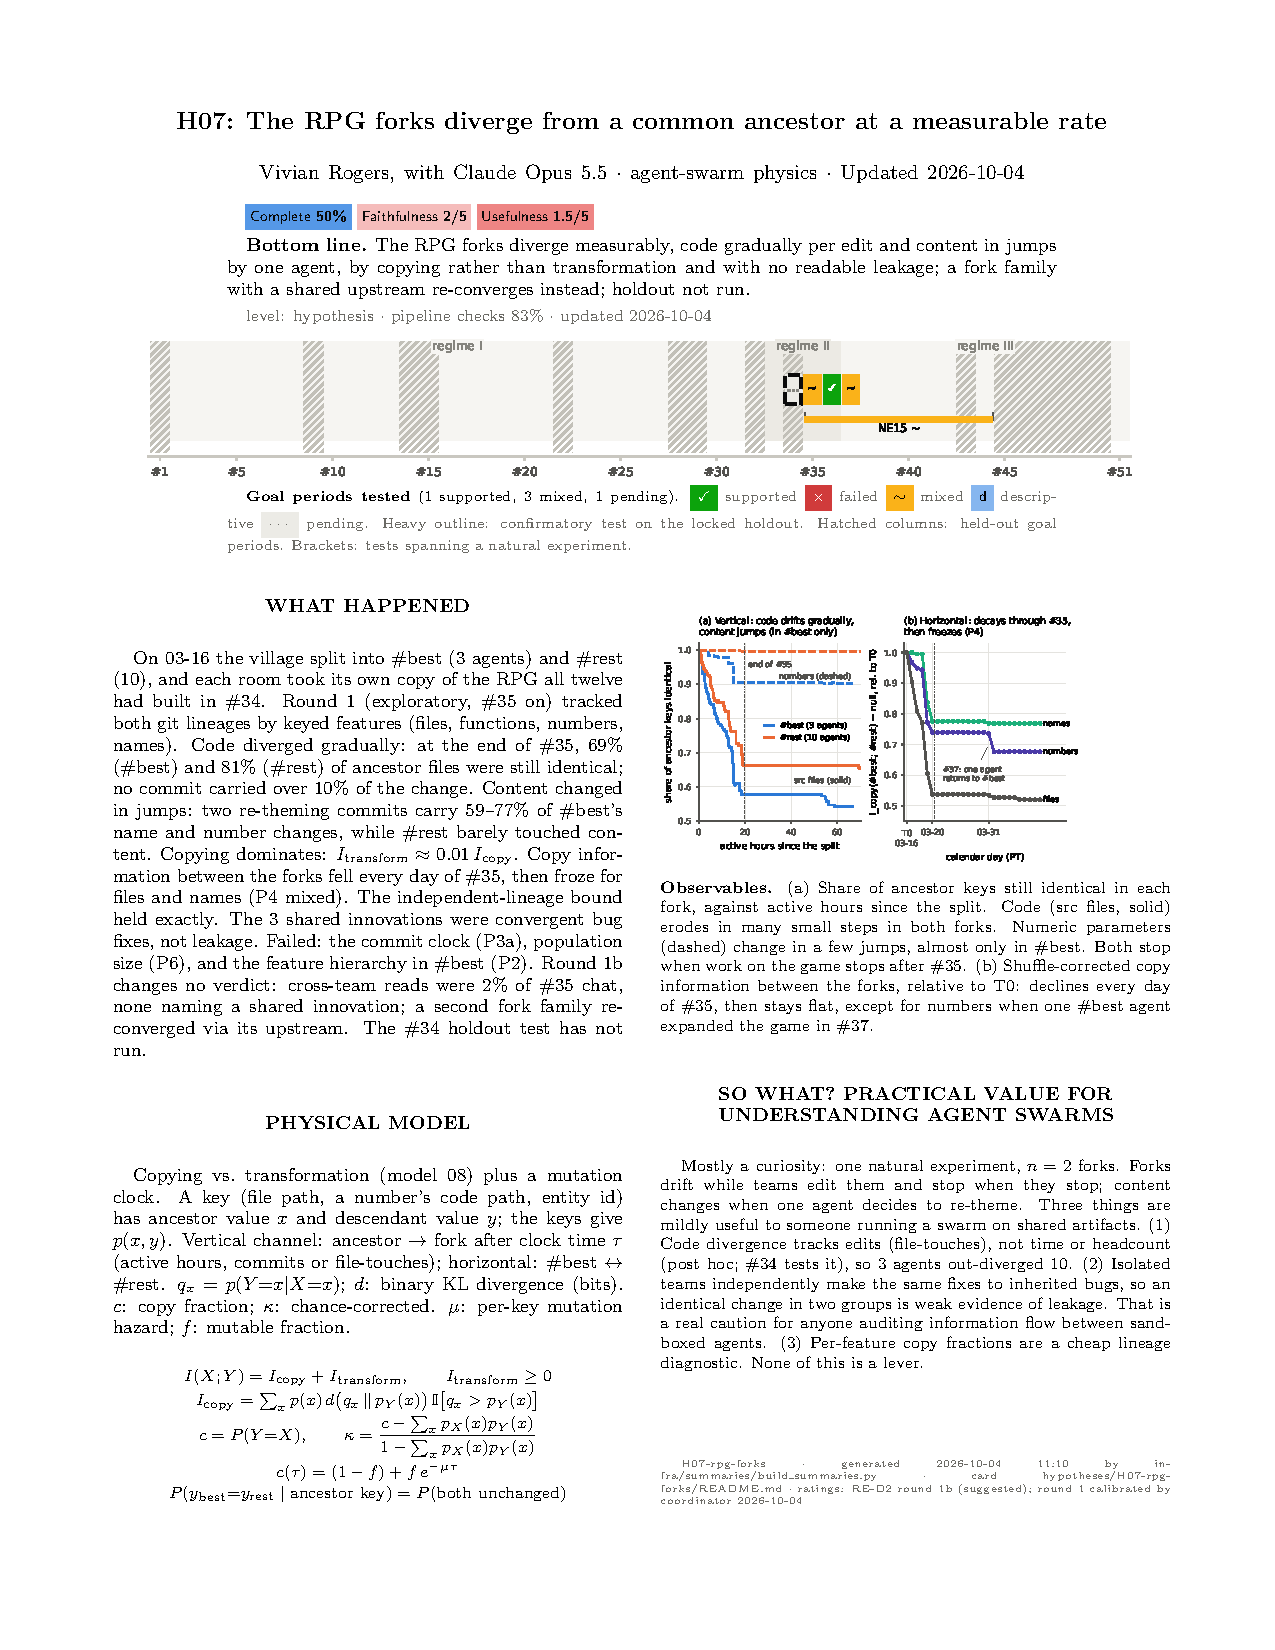
\includepdf[pages=1,link,linkname=H07]{../../hypotheses/H07-rpg-forks/summary/summary.pdf}
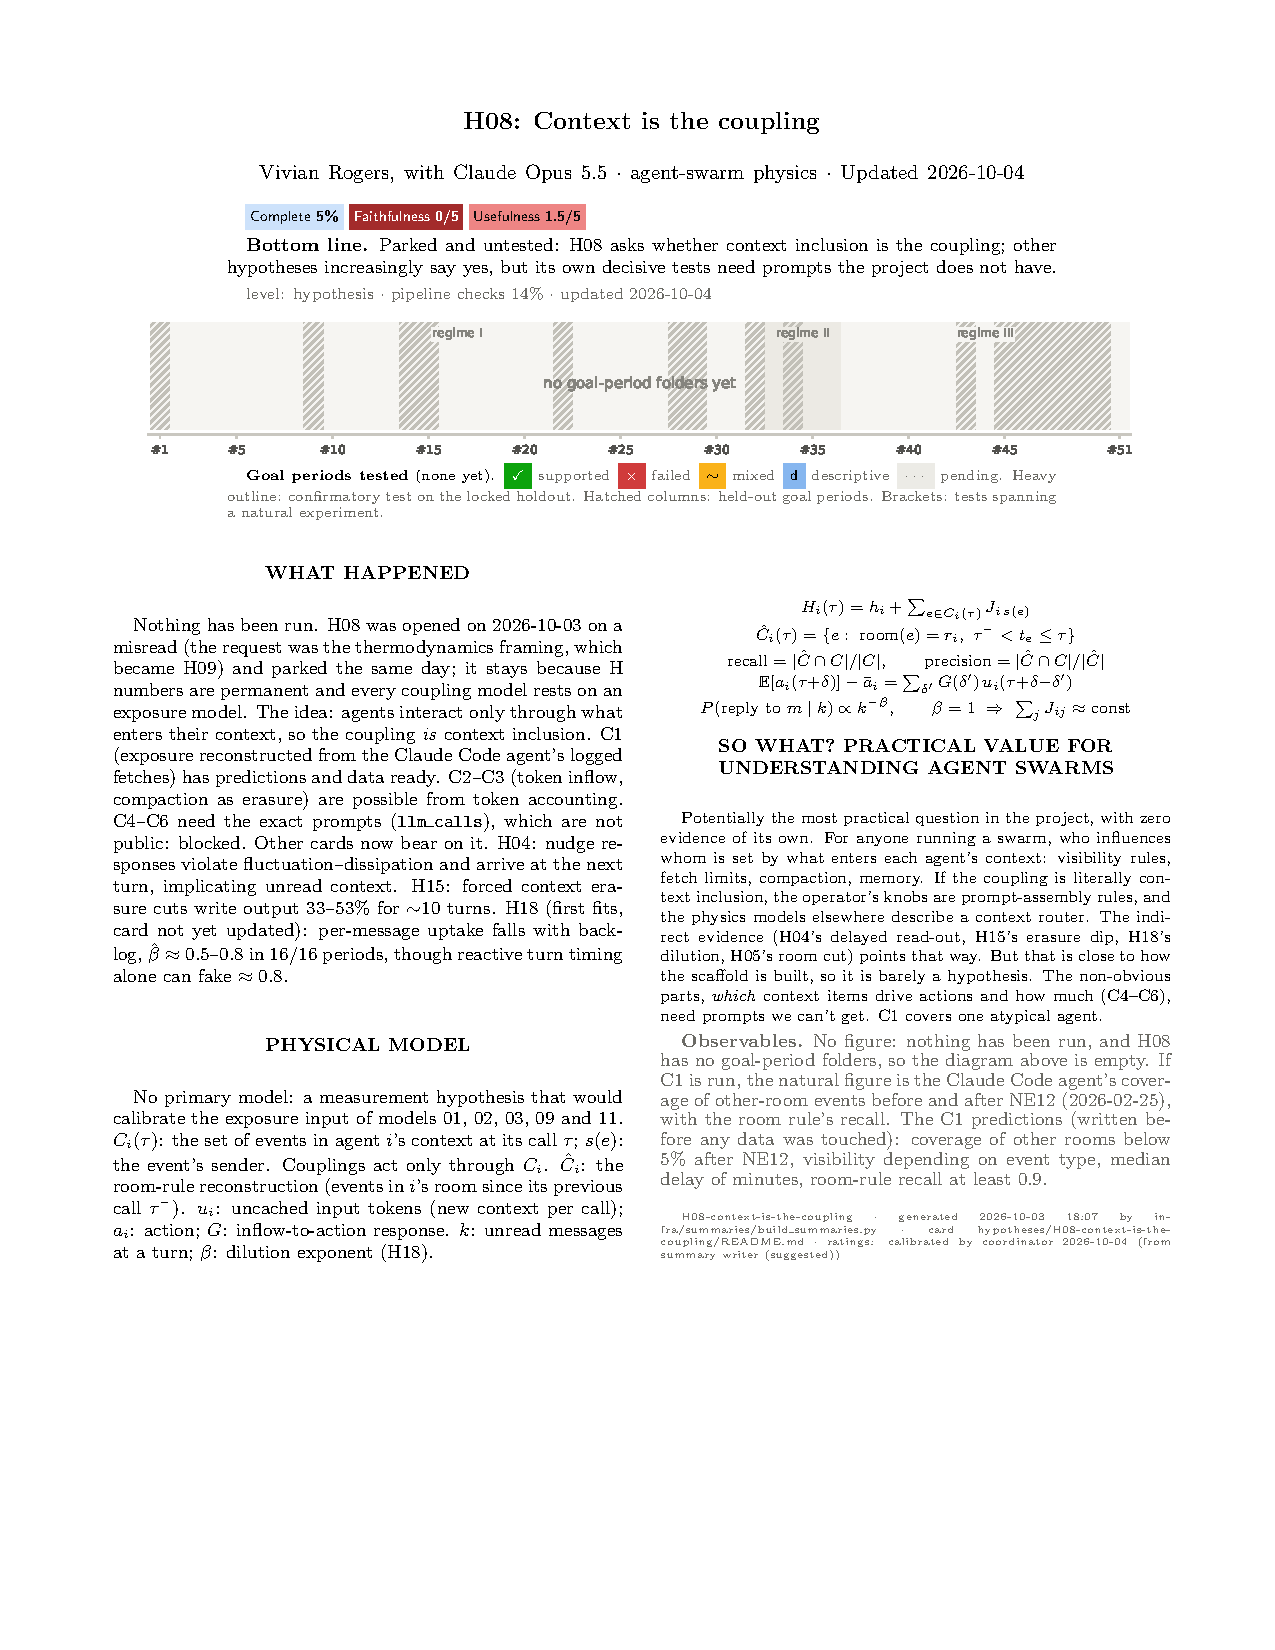
\includepdf[pages=1,link,linkname=H08]{../../hypotheses/H08-context-is-the-coupling/summary/summary.pdf}
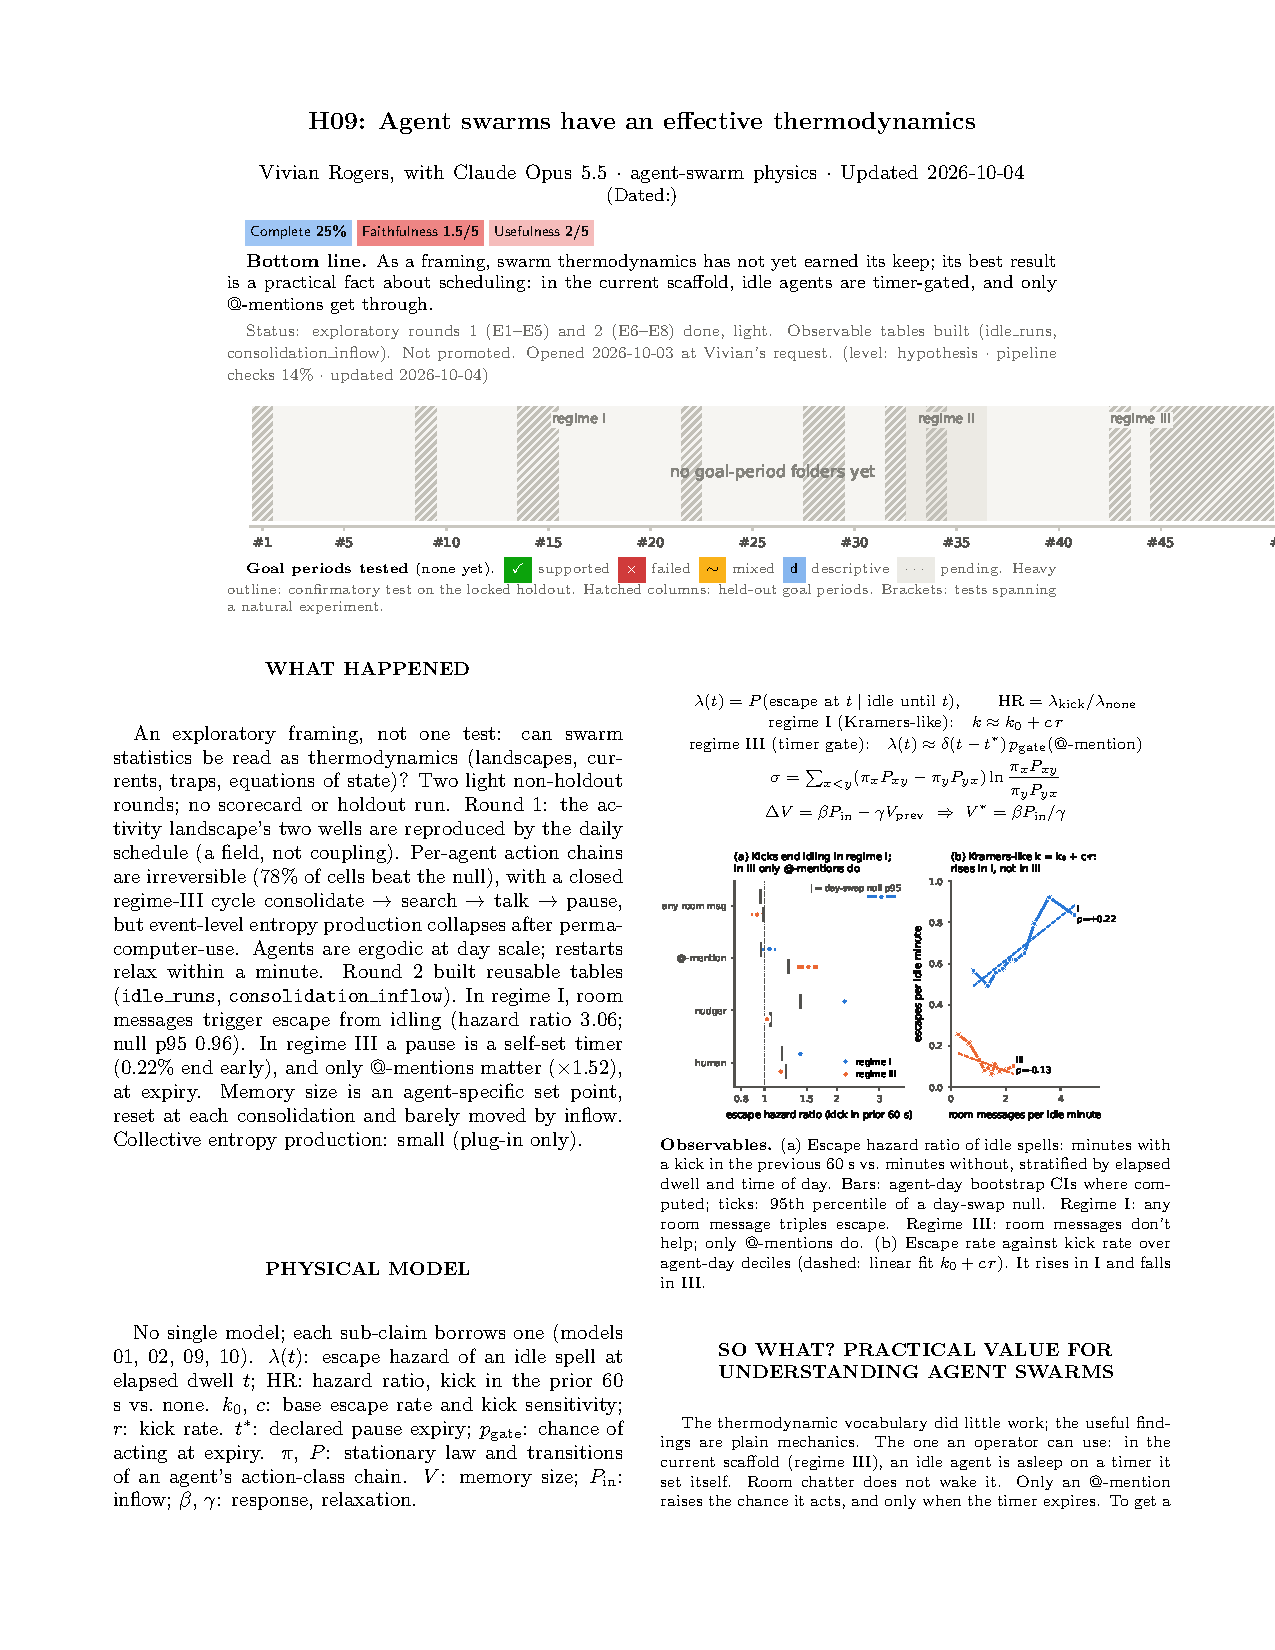
\includepdf[pages=1,link,linkname=H09]{../../hypotheses/H09-swarm-thermodynamics/summary/summary.pdf}
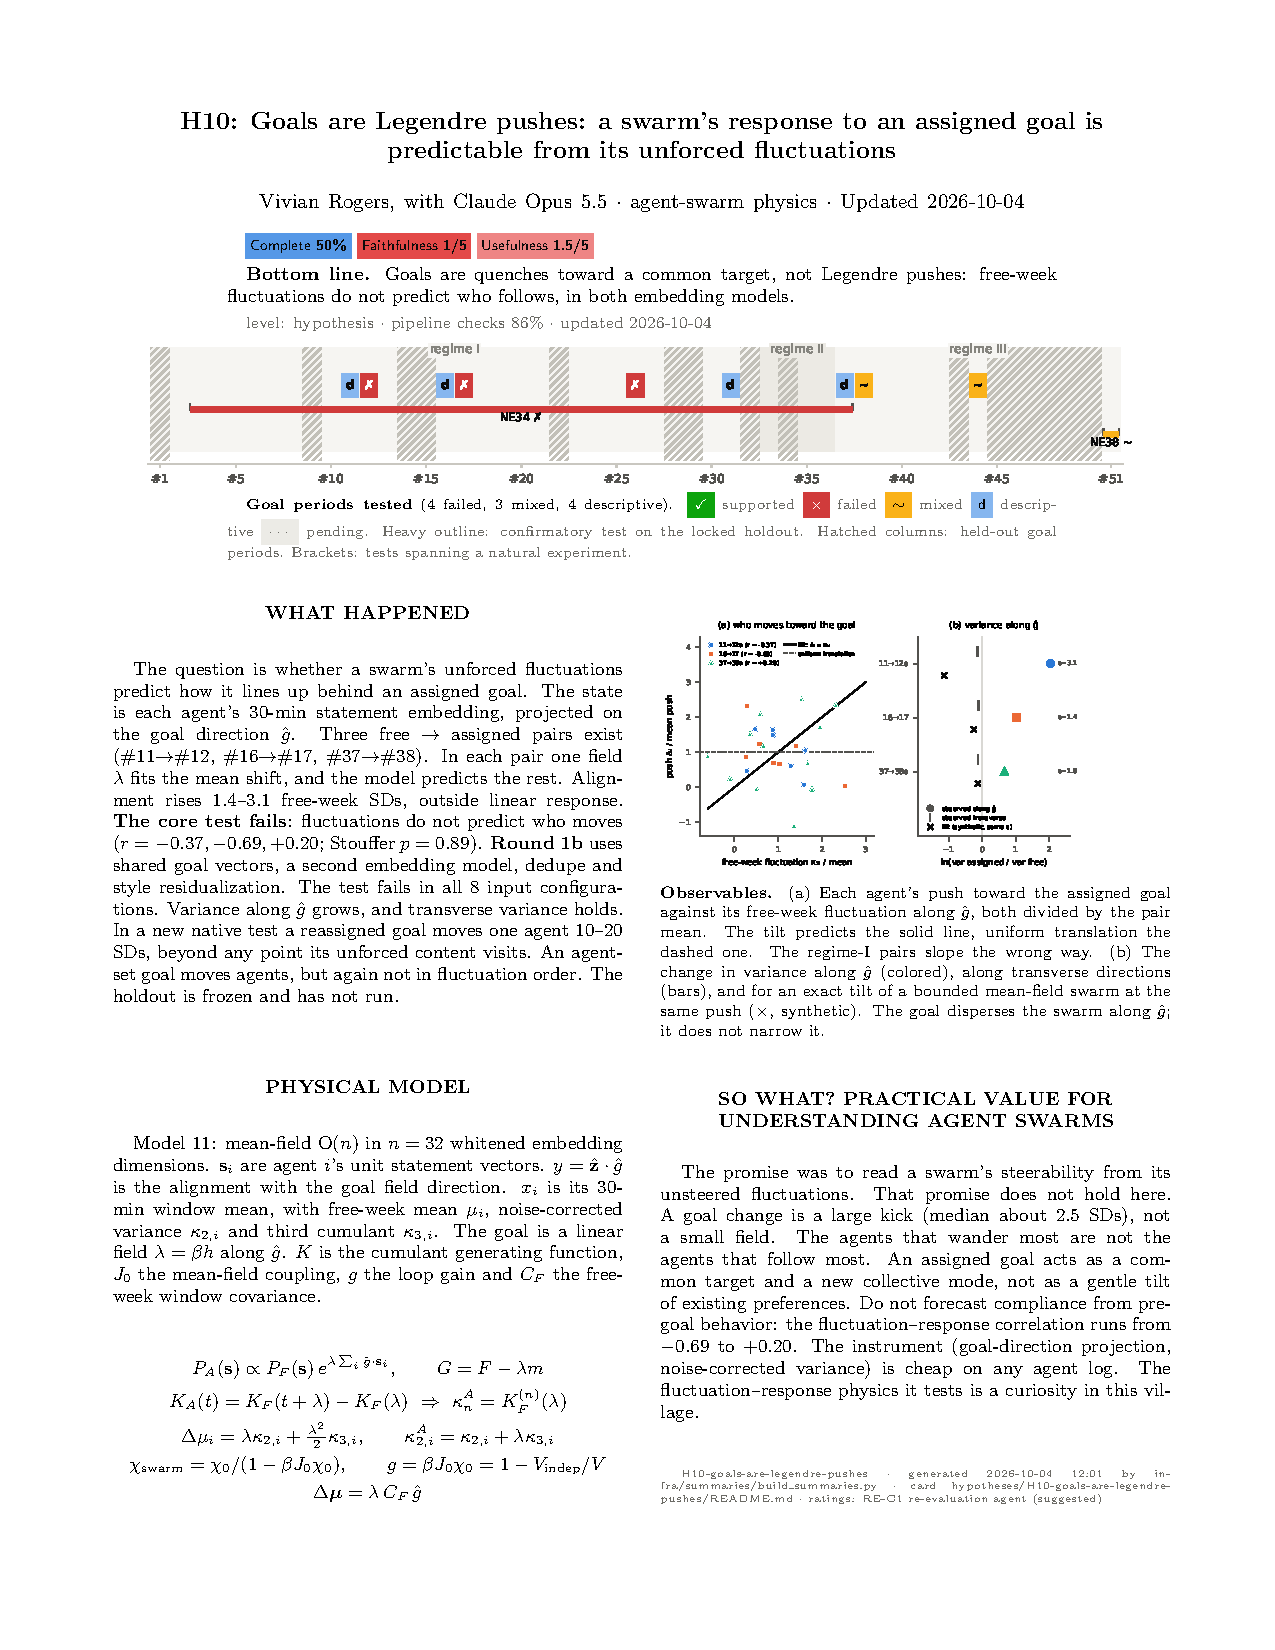
\includepdf[pages=1,link,linkname=H10]{../../hypotheses/H10-goals-are-legendre-pushes/summary/summary.pdf}
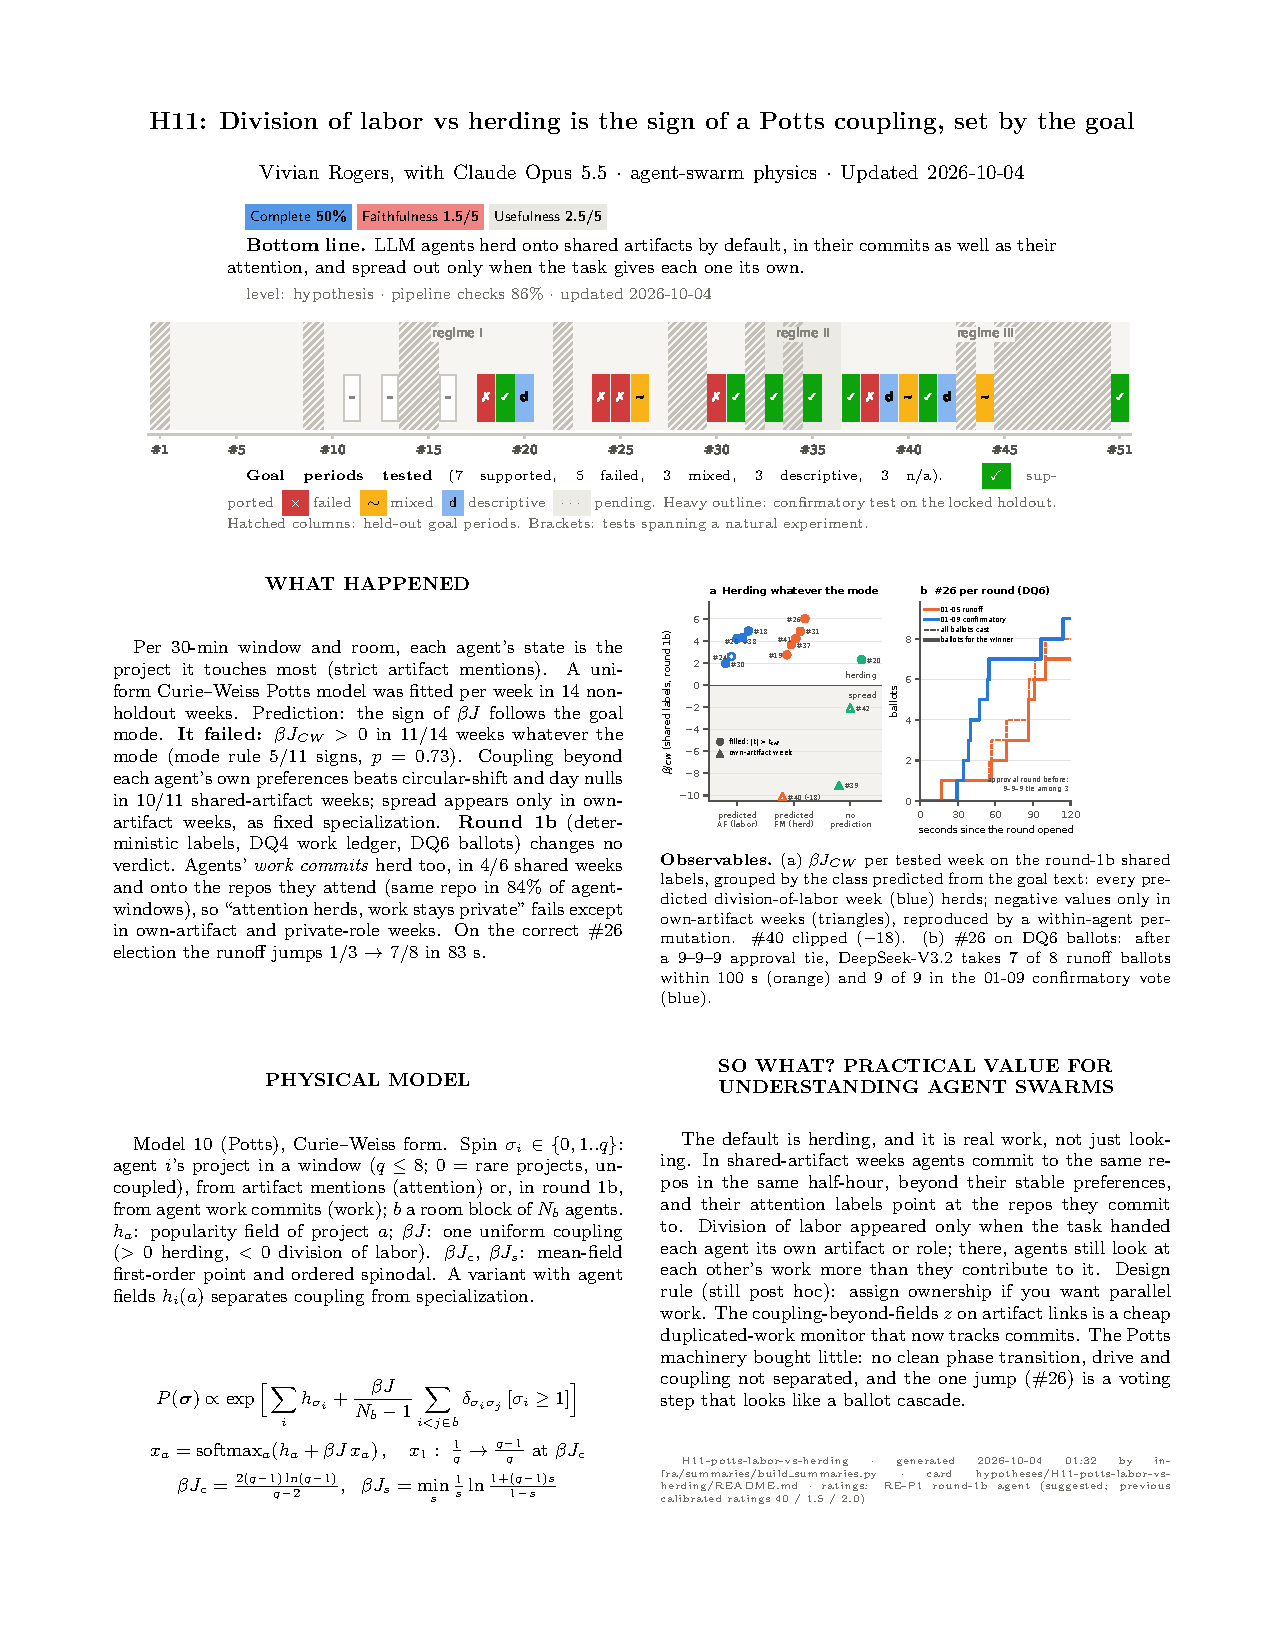
\includepdf[pages=1,link,linkname=H11]{../../hypotheses/H11-potts-labor-vs-herding/summary/summary.pdf}
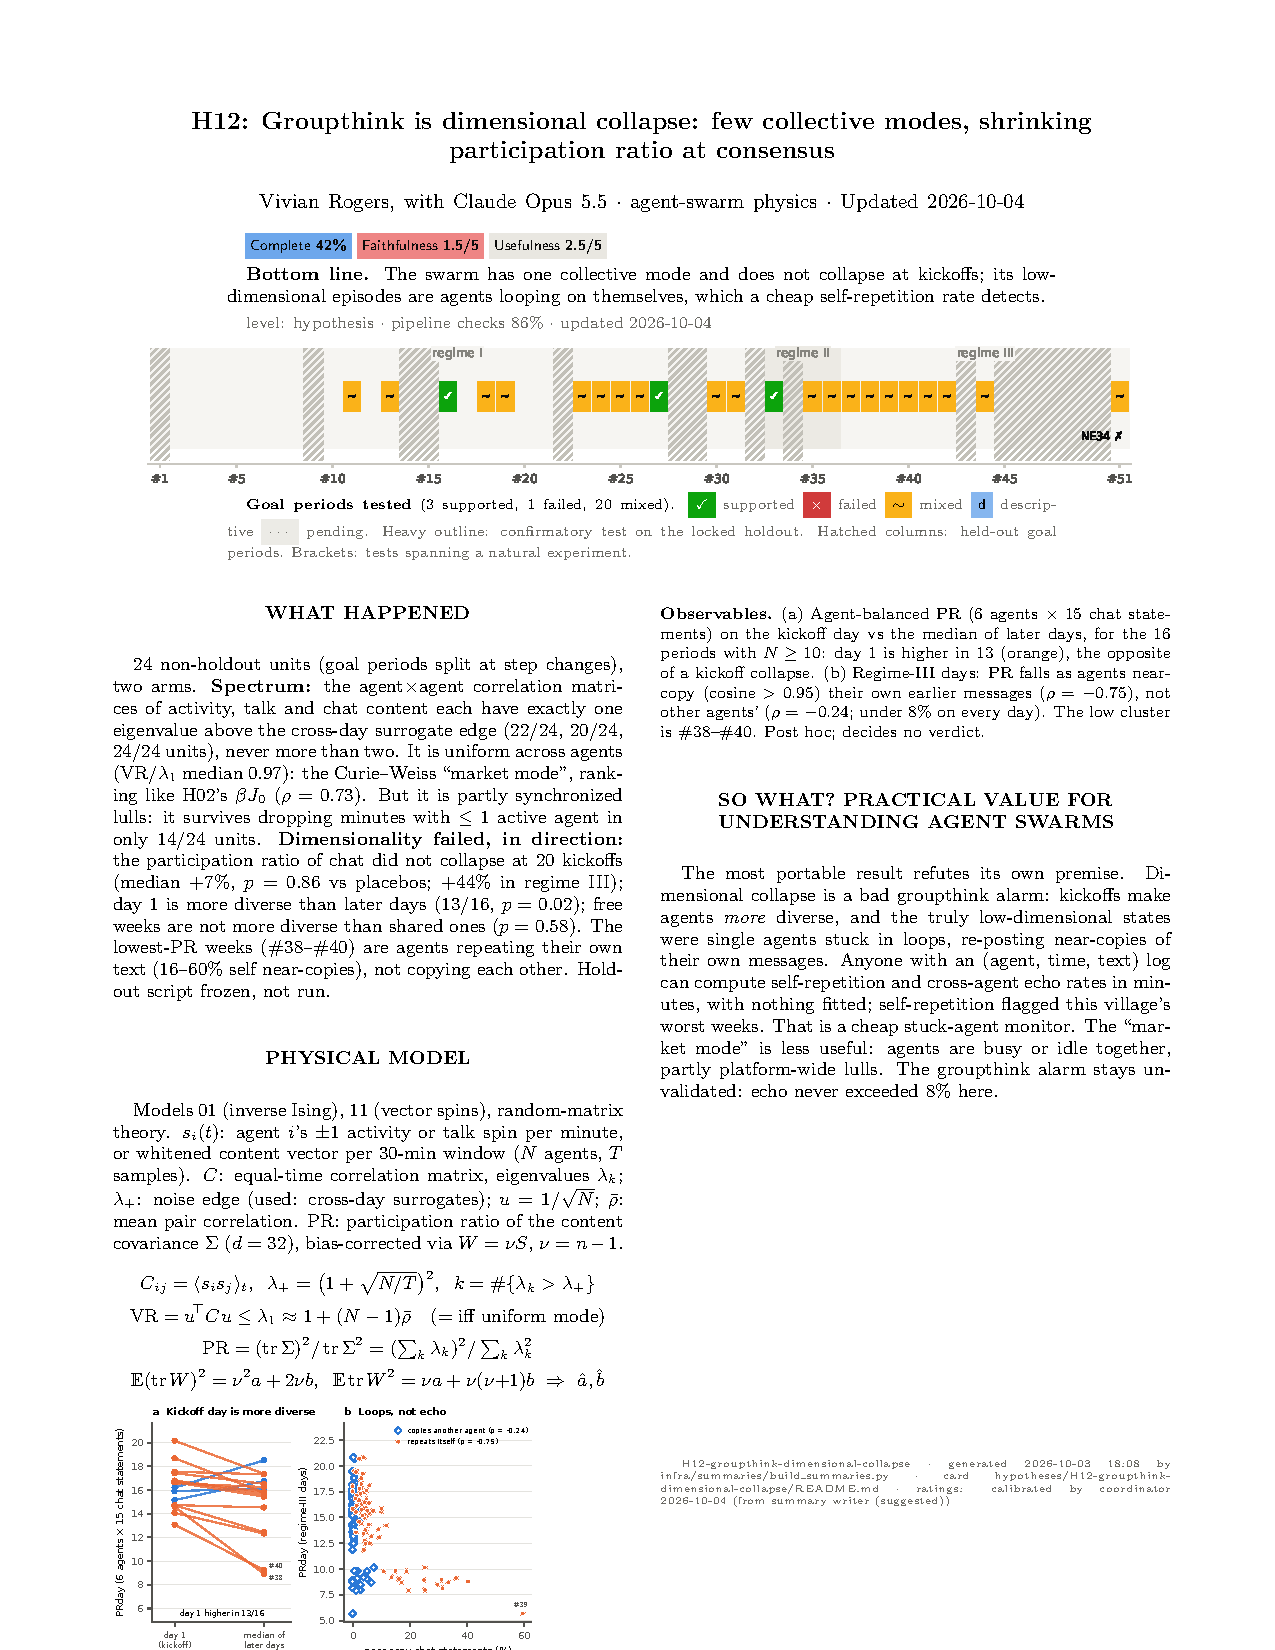
\includepdf[pages=1,link,linkname=H12]{../../hypotheses/H12-groupthink-dimensional-collapse/summary/summary.pdf}
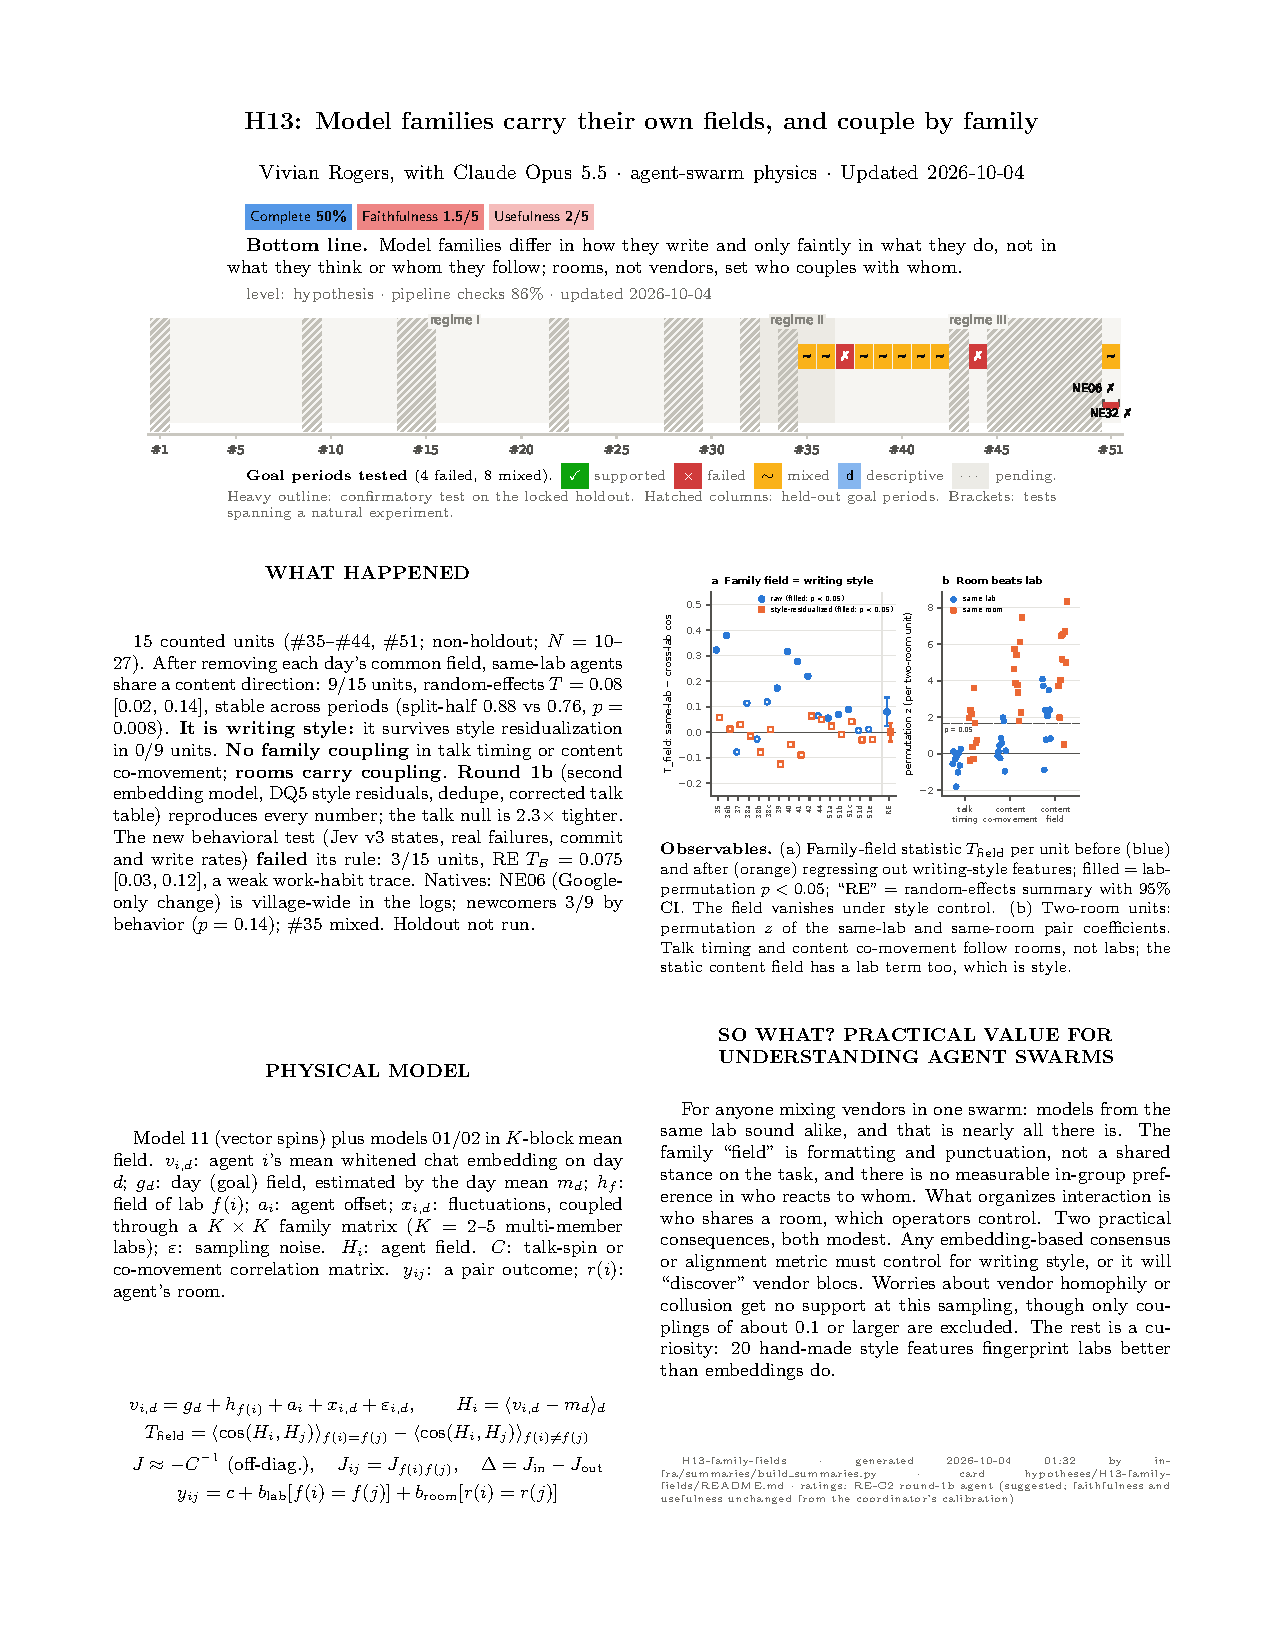
\includepdf[pages=1,link,linkname=H13]{../../hypotheses/H13-family-fields/summary/summary.pdf}
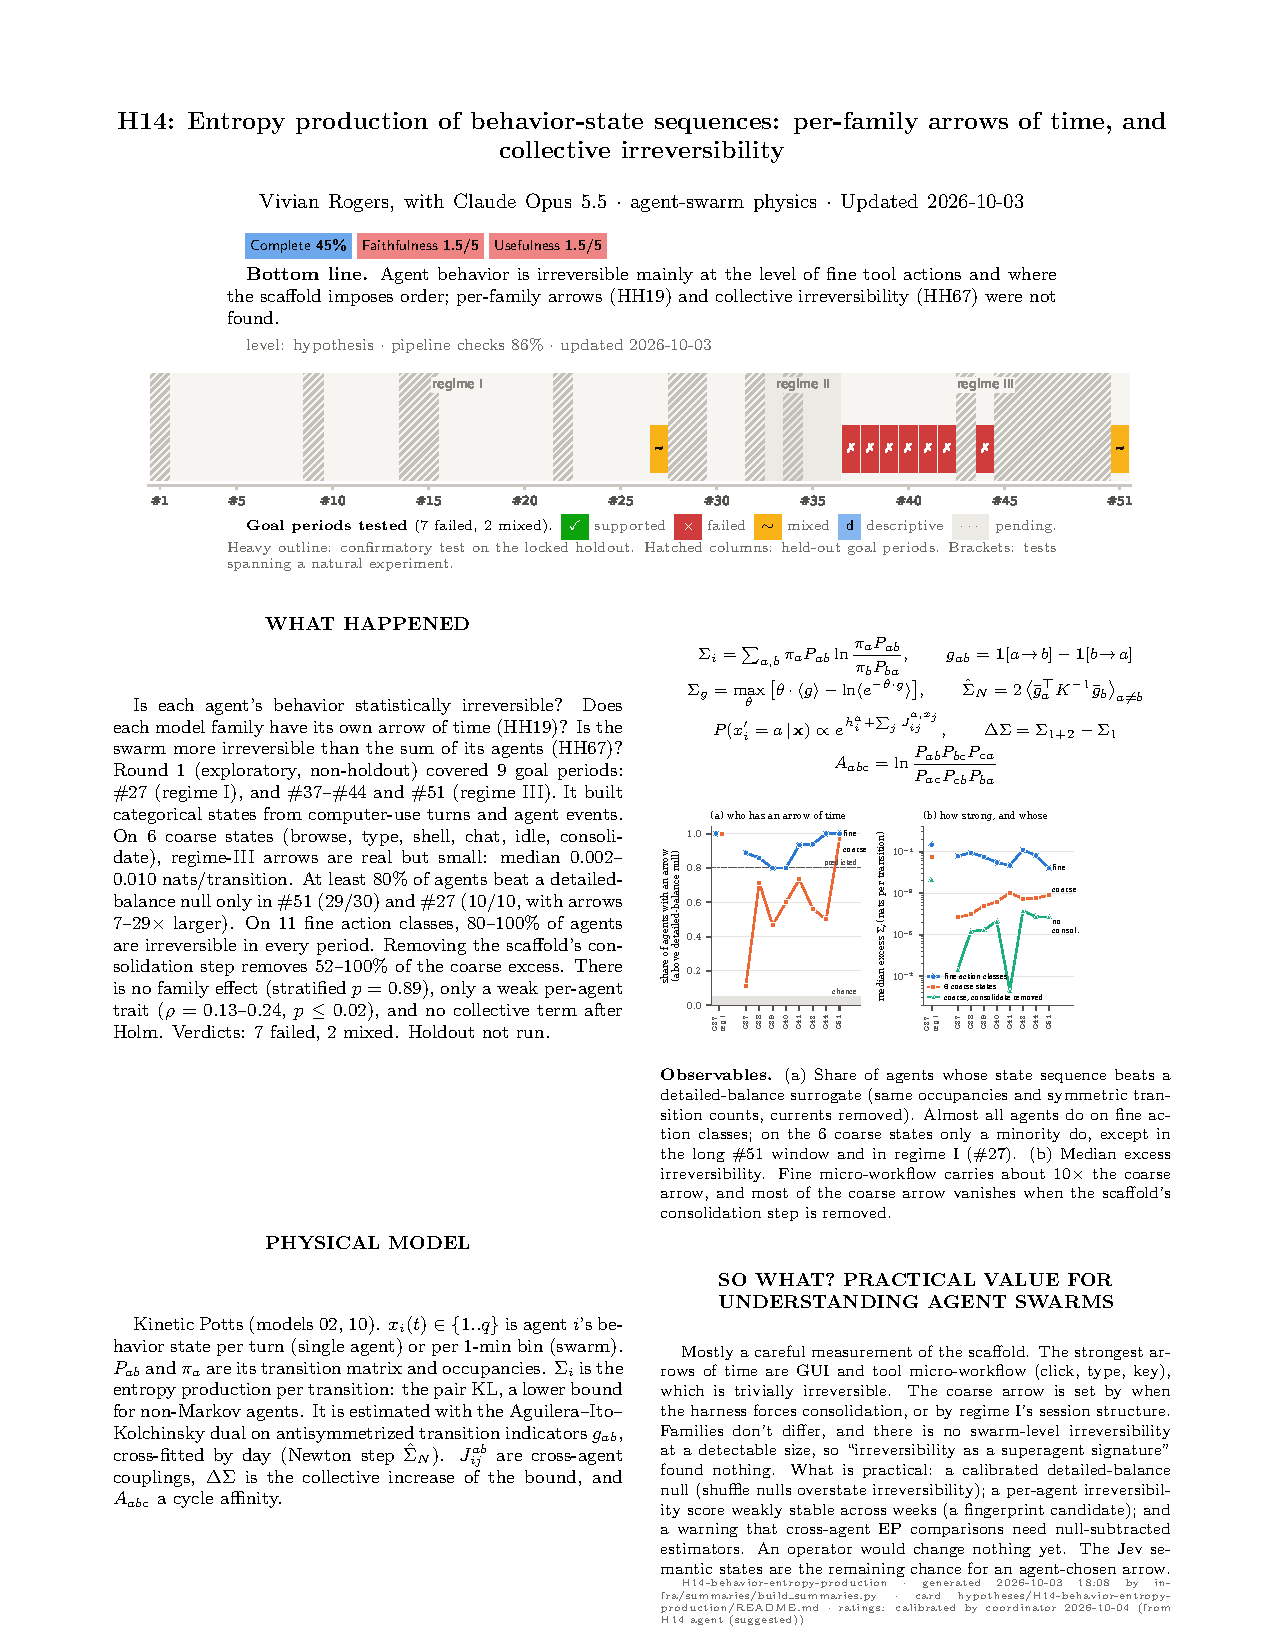
\includepdf[pages=1,link,linkname=H14]{../../hypotheses/H14-behavior-entropy-production/summary/summary.pdf}
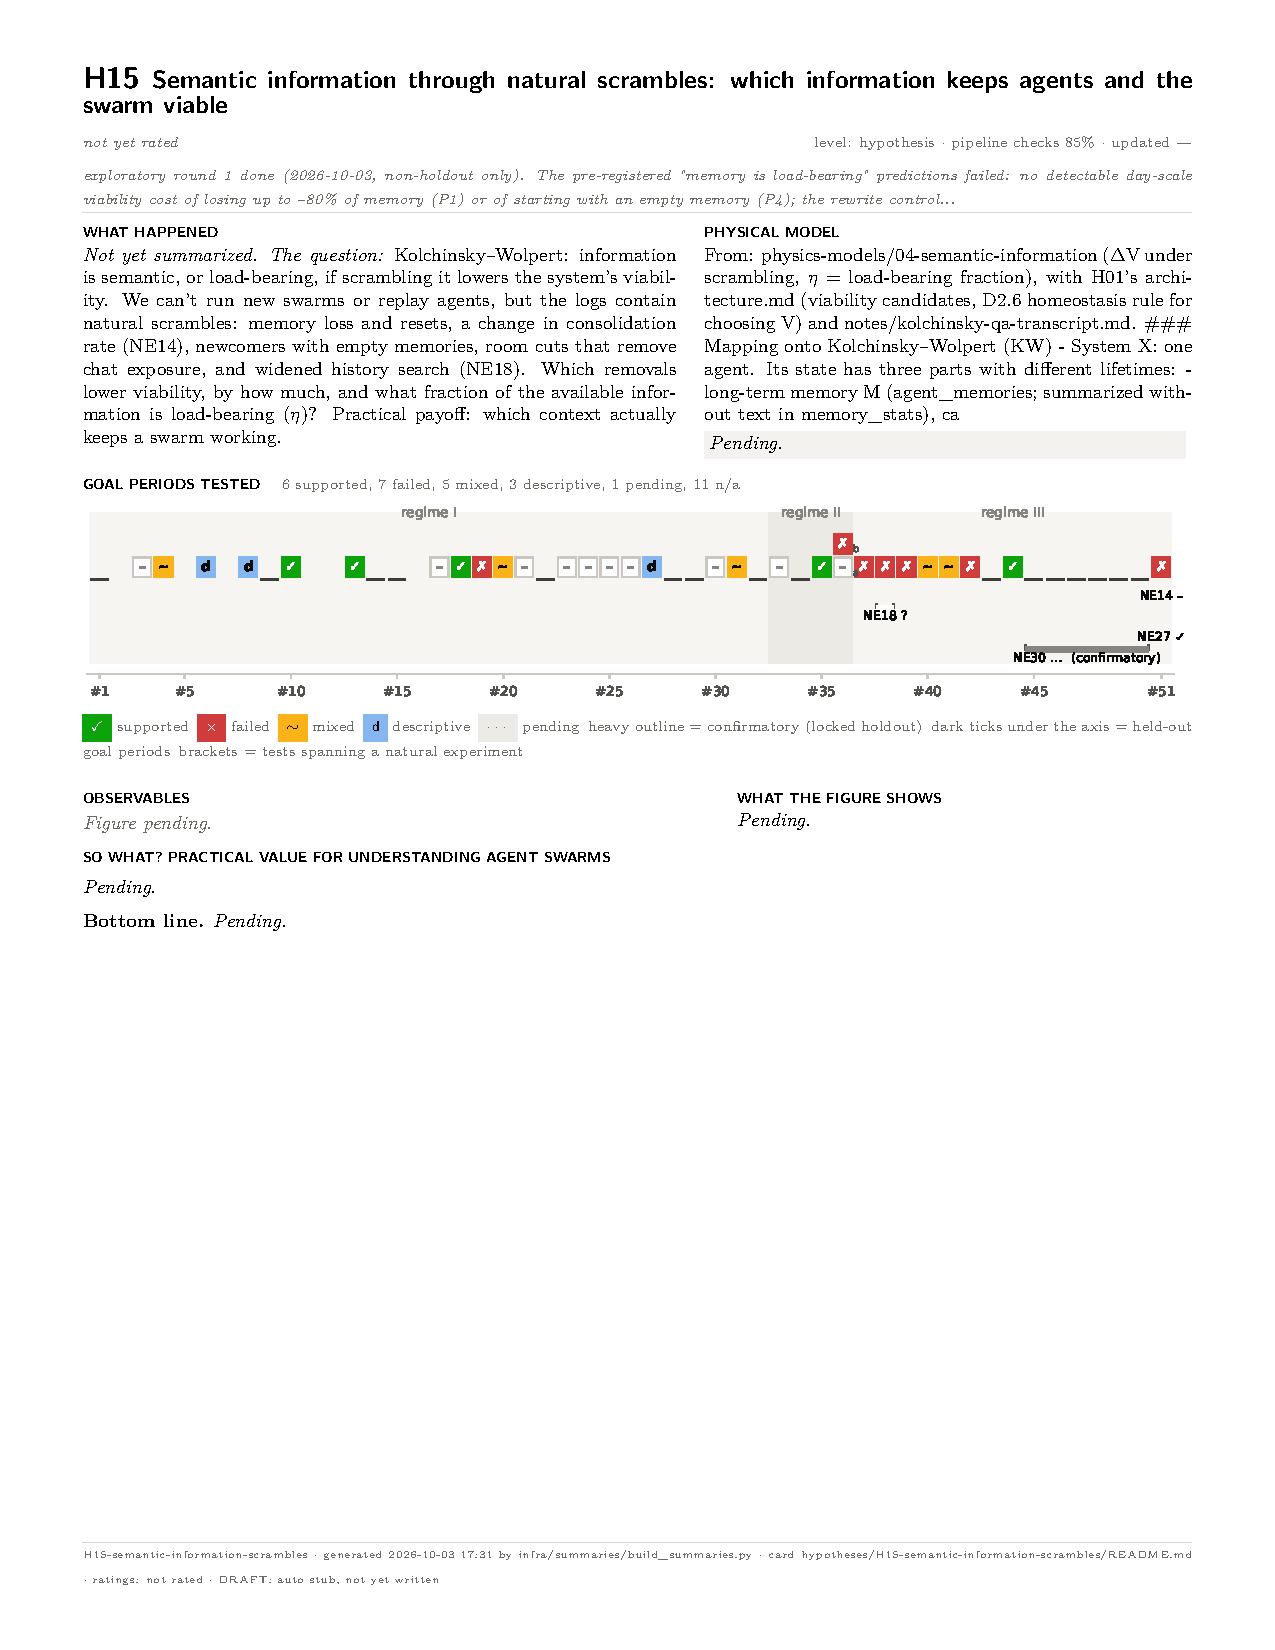
\includepdf[pages=1,link,linkname=H15]{../../hypotheses/H15-semantic-information-scrambles/summary/summary.pdf}
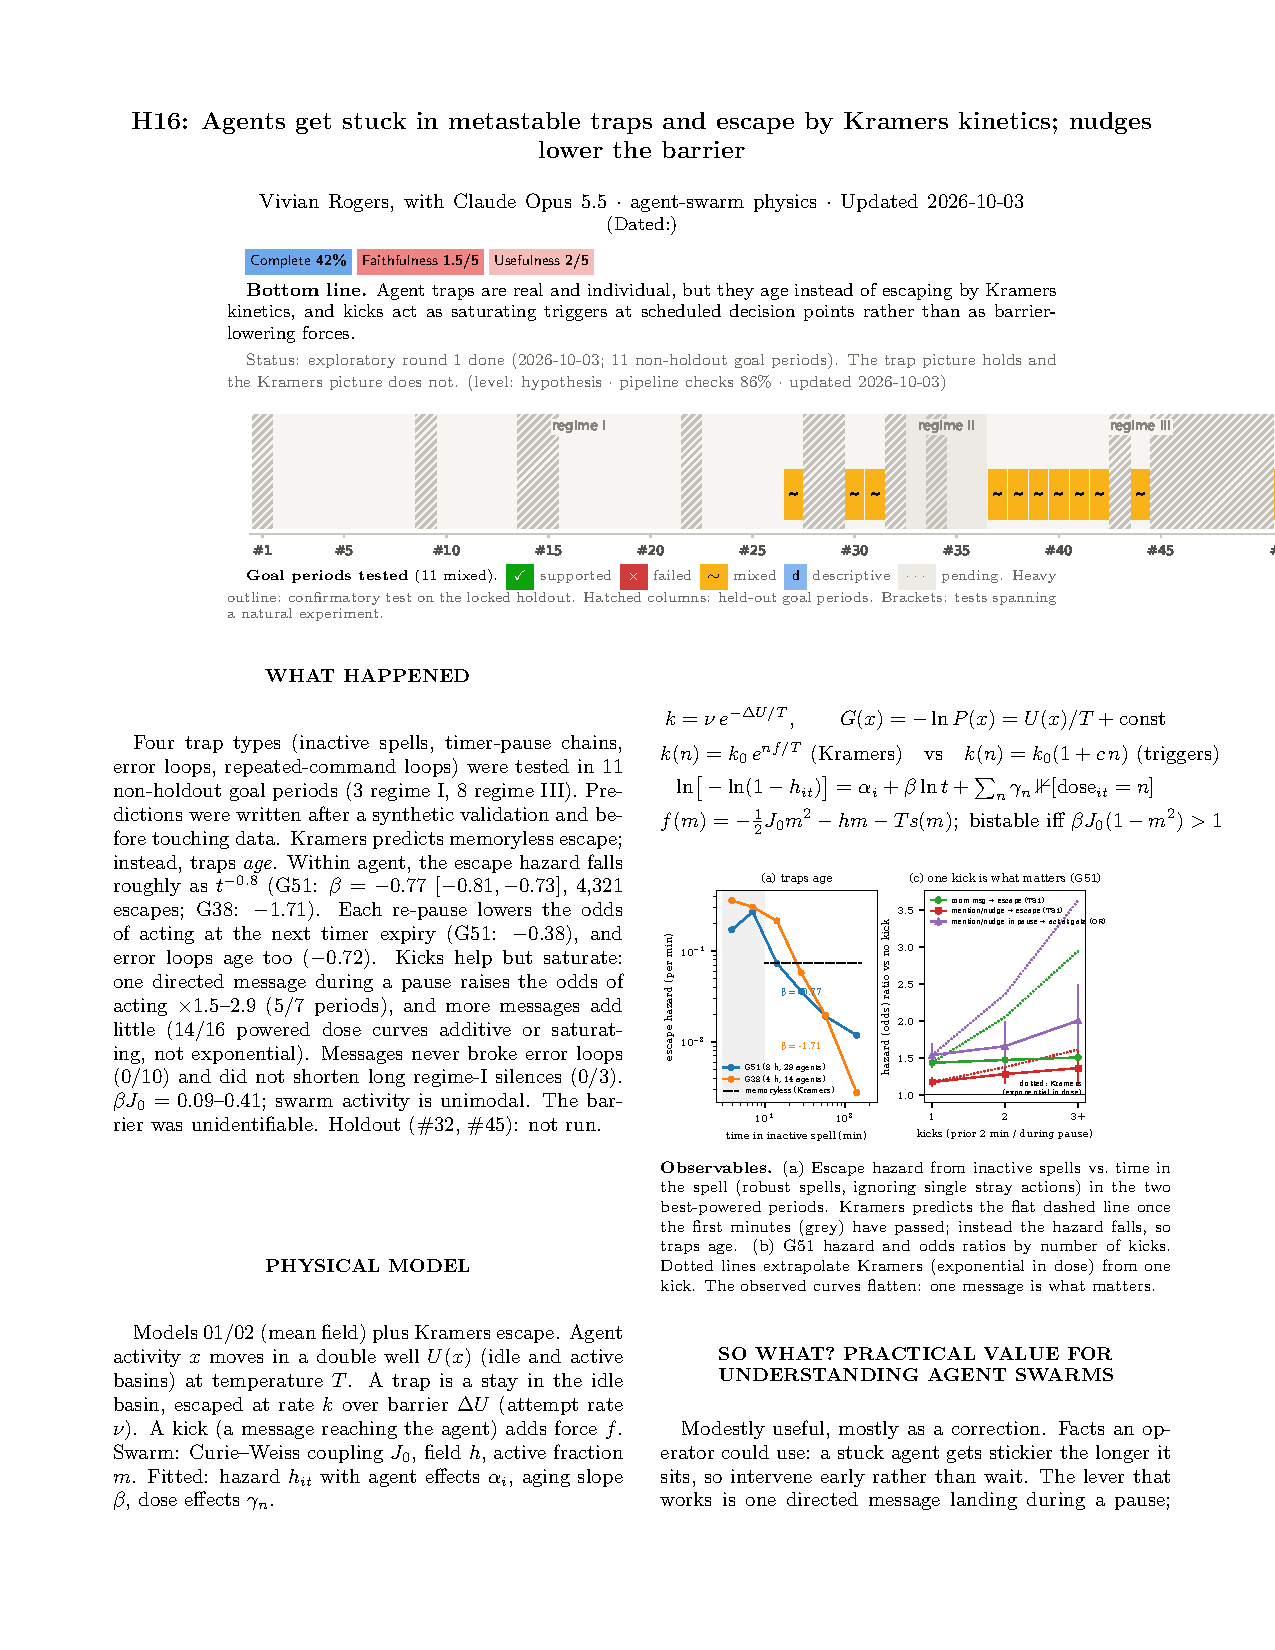
\includepdf[pages=1,link,linkname=H16]{../../hypotheses/H16-metastable-traps-kramers/summary/summary.pdf}
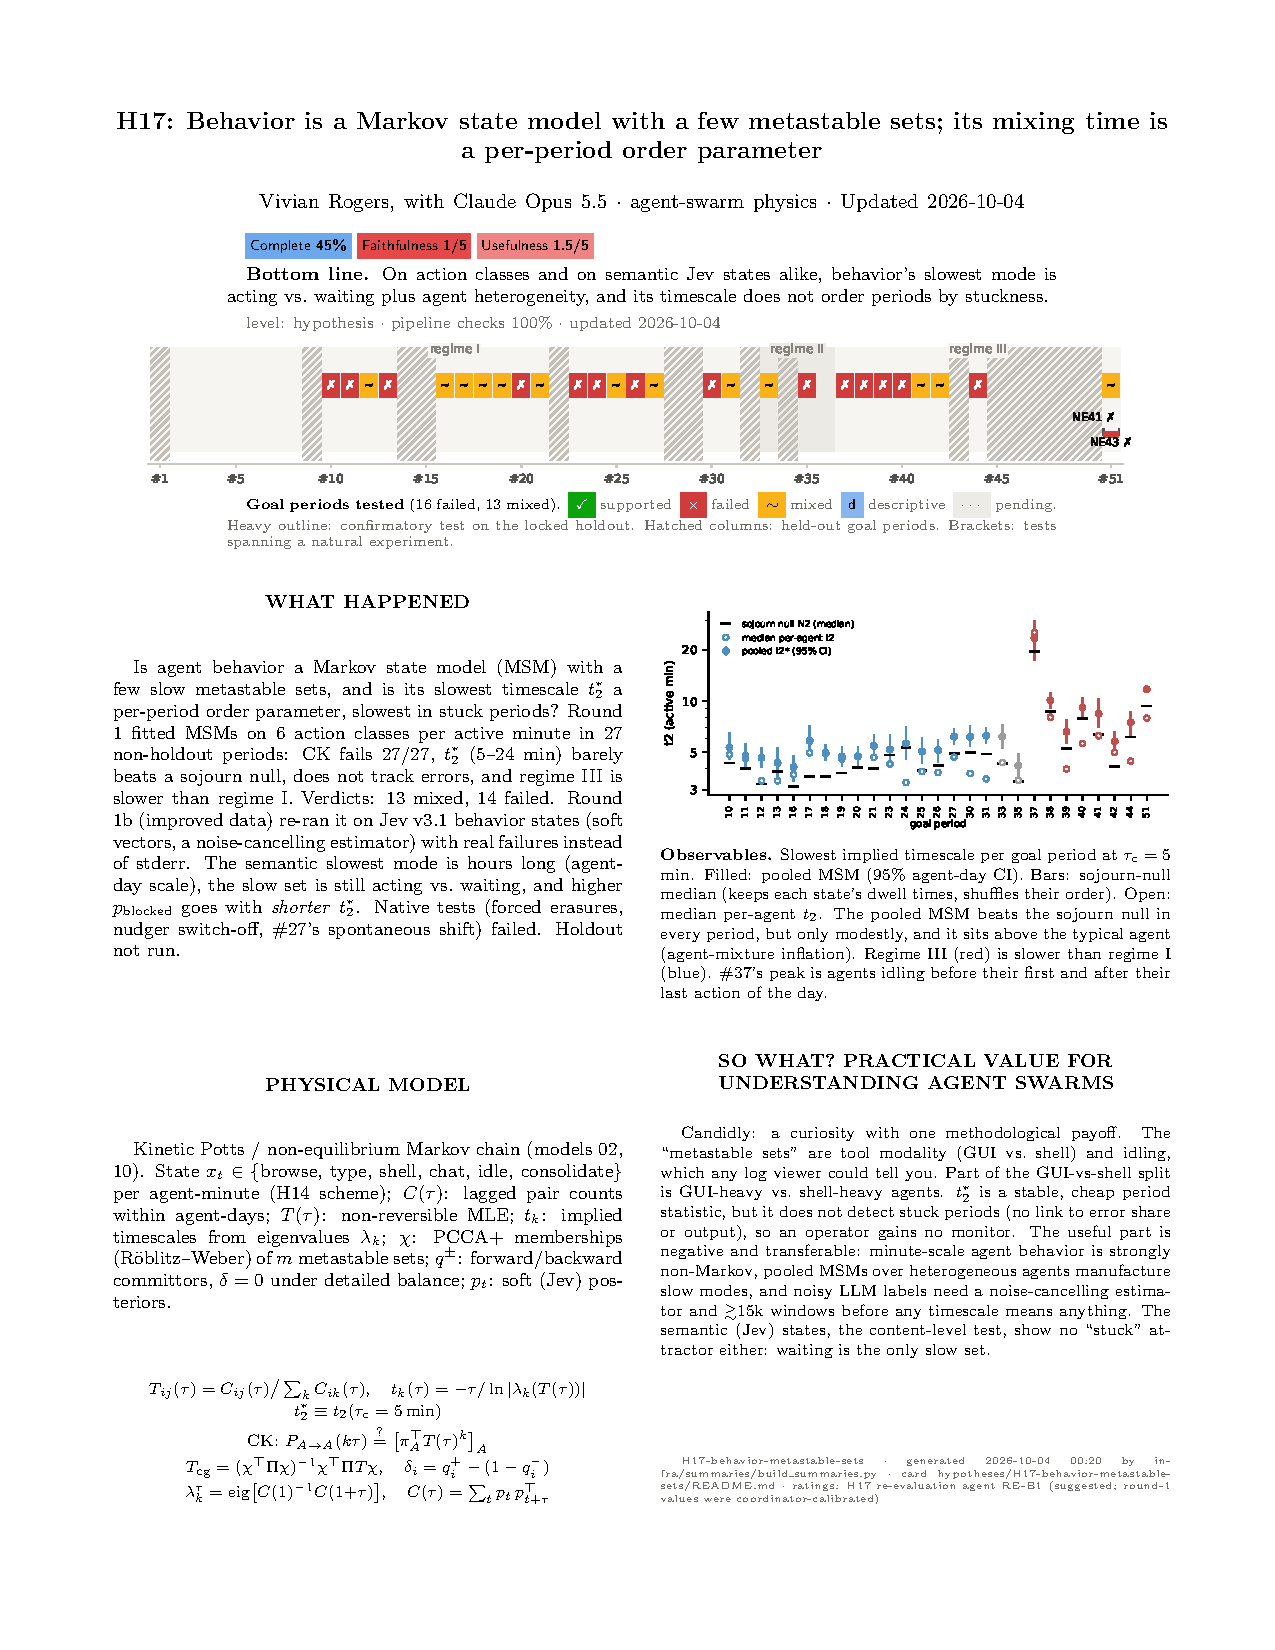
\includepdf[pages=1,link,linkname=H17]{../../hypotheses/H17-behavior-metastable-sets/summary/summary.pdf}
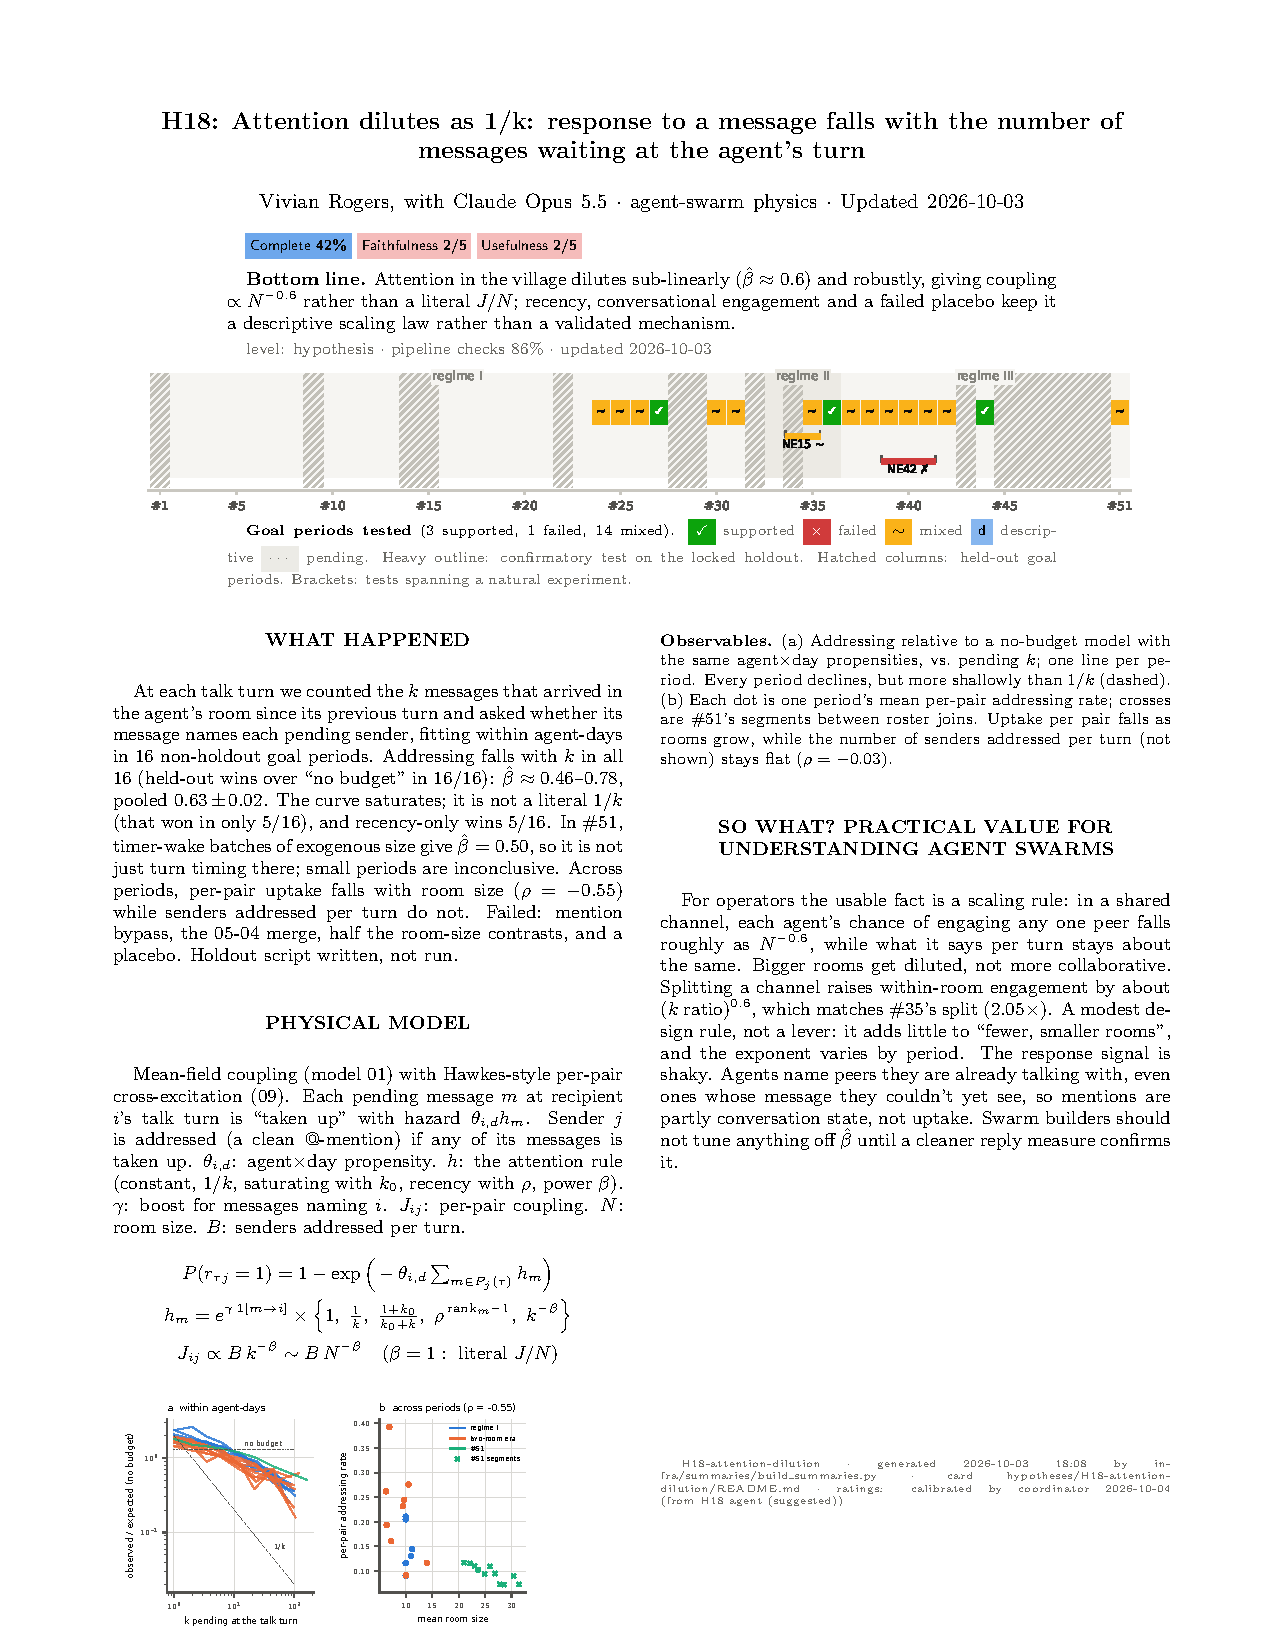
\includepdf[pages=1,link,linkname=H18]{../../hypotheses/H18-attention-dilution/summary/summary.pdf}
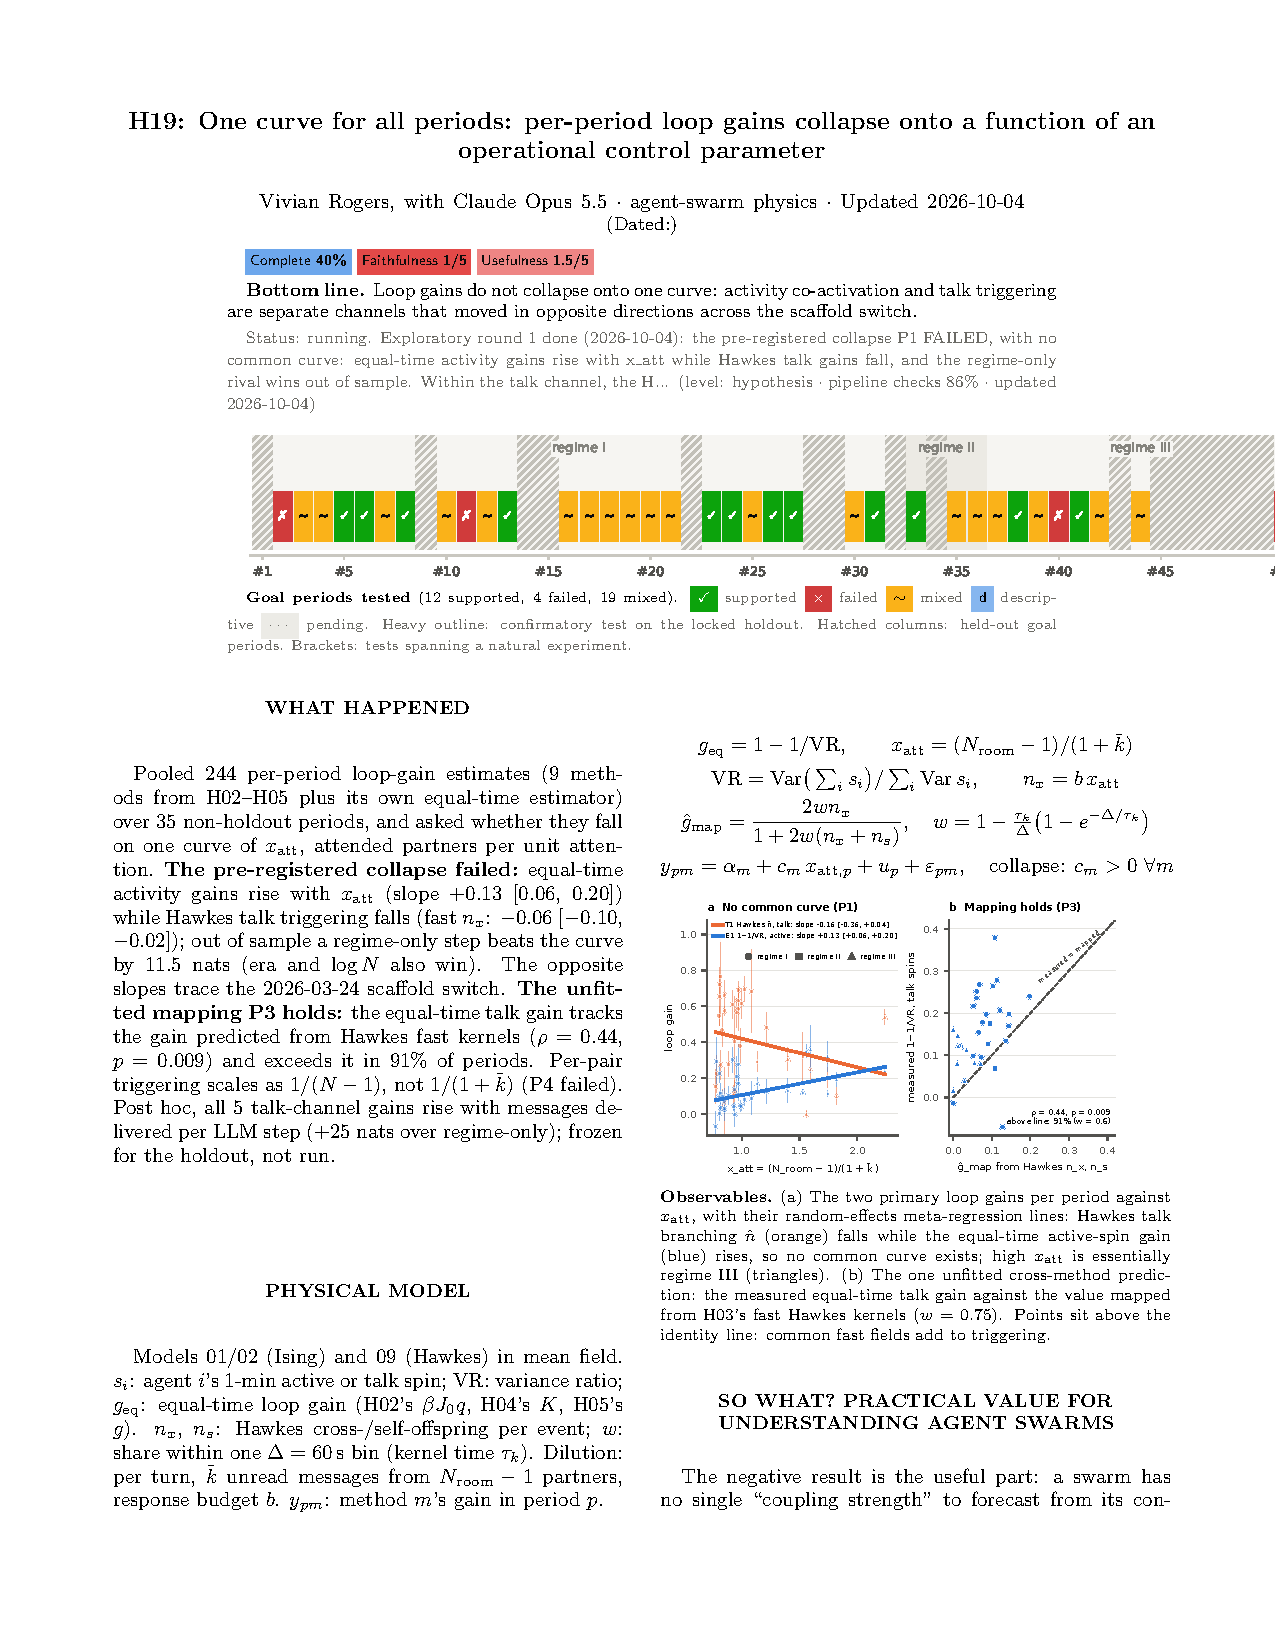
\includepdf[pages=1,link,linkname=H19]{../../hypotheses/H19-loop-gain-collapse/summary/summary.pdf}
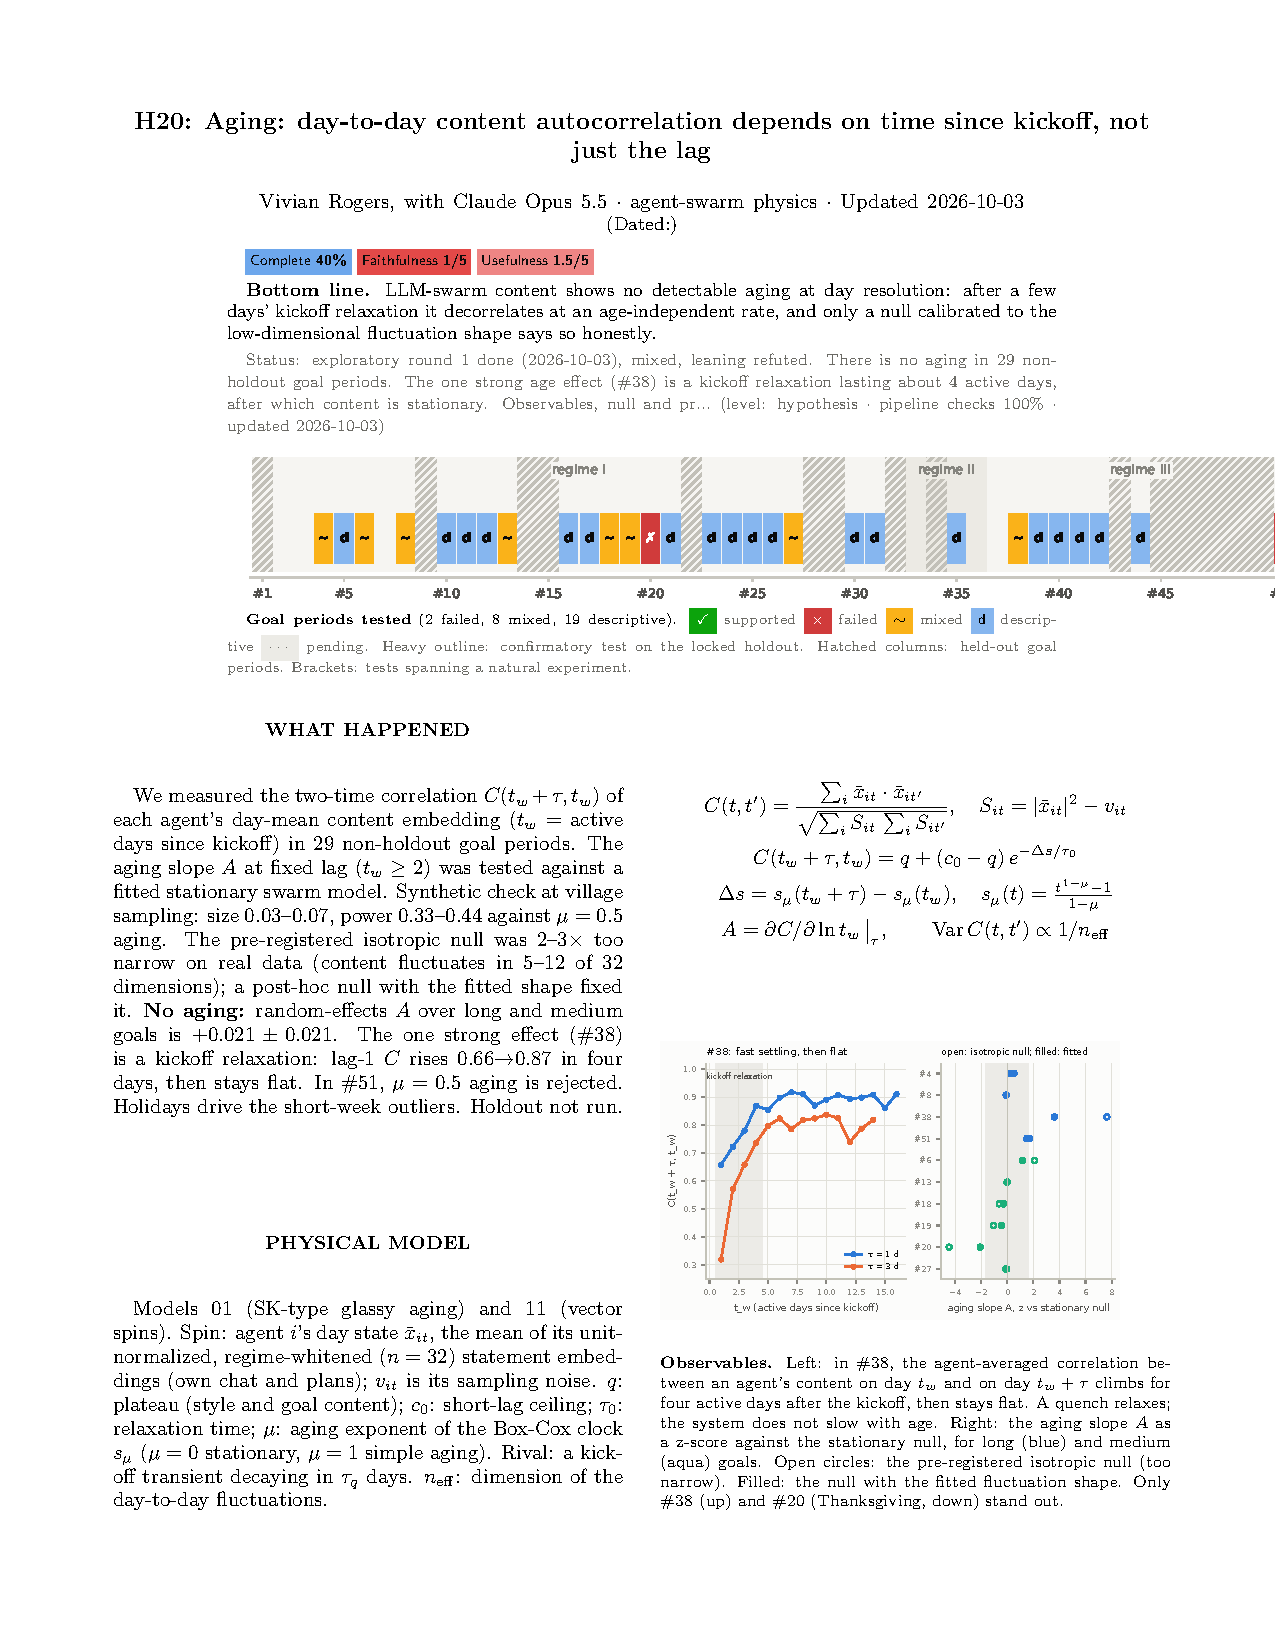
\includepdf[pages=1,link,linkname=H20]{../../hypotheses/H20-content-aging/summary/summary.pdf}
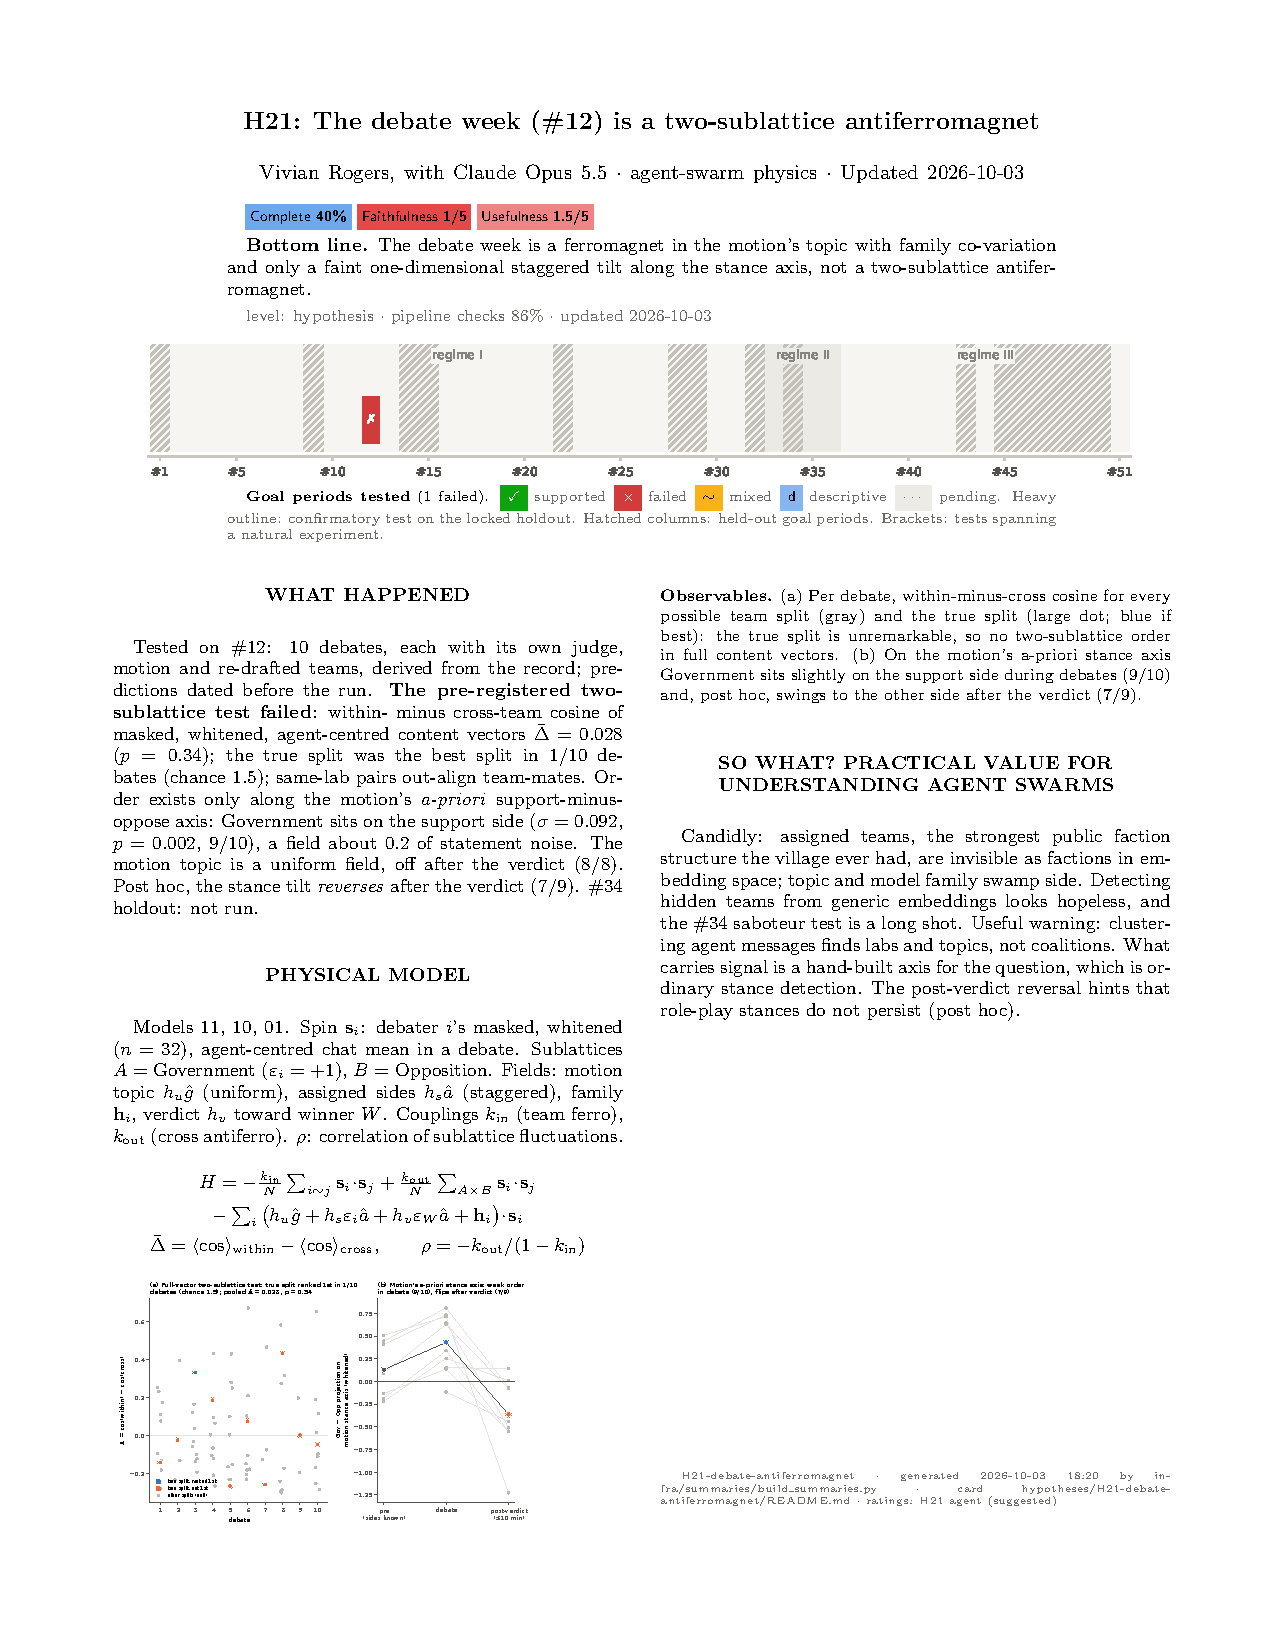
\includepdf[pages=1,link,linkname=H21]{../../hypotheses/H21-debate-antiferromagnet/summary/summary.pdf}
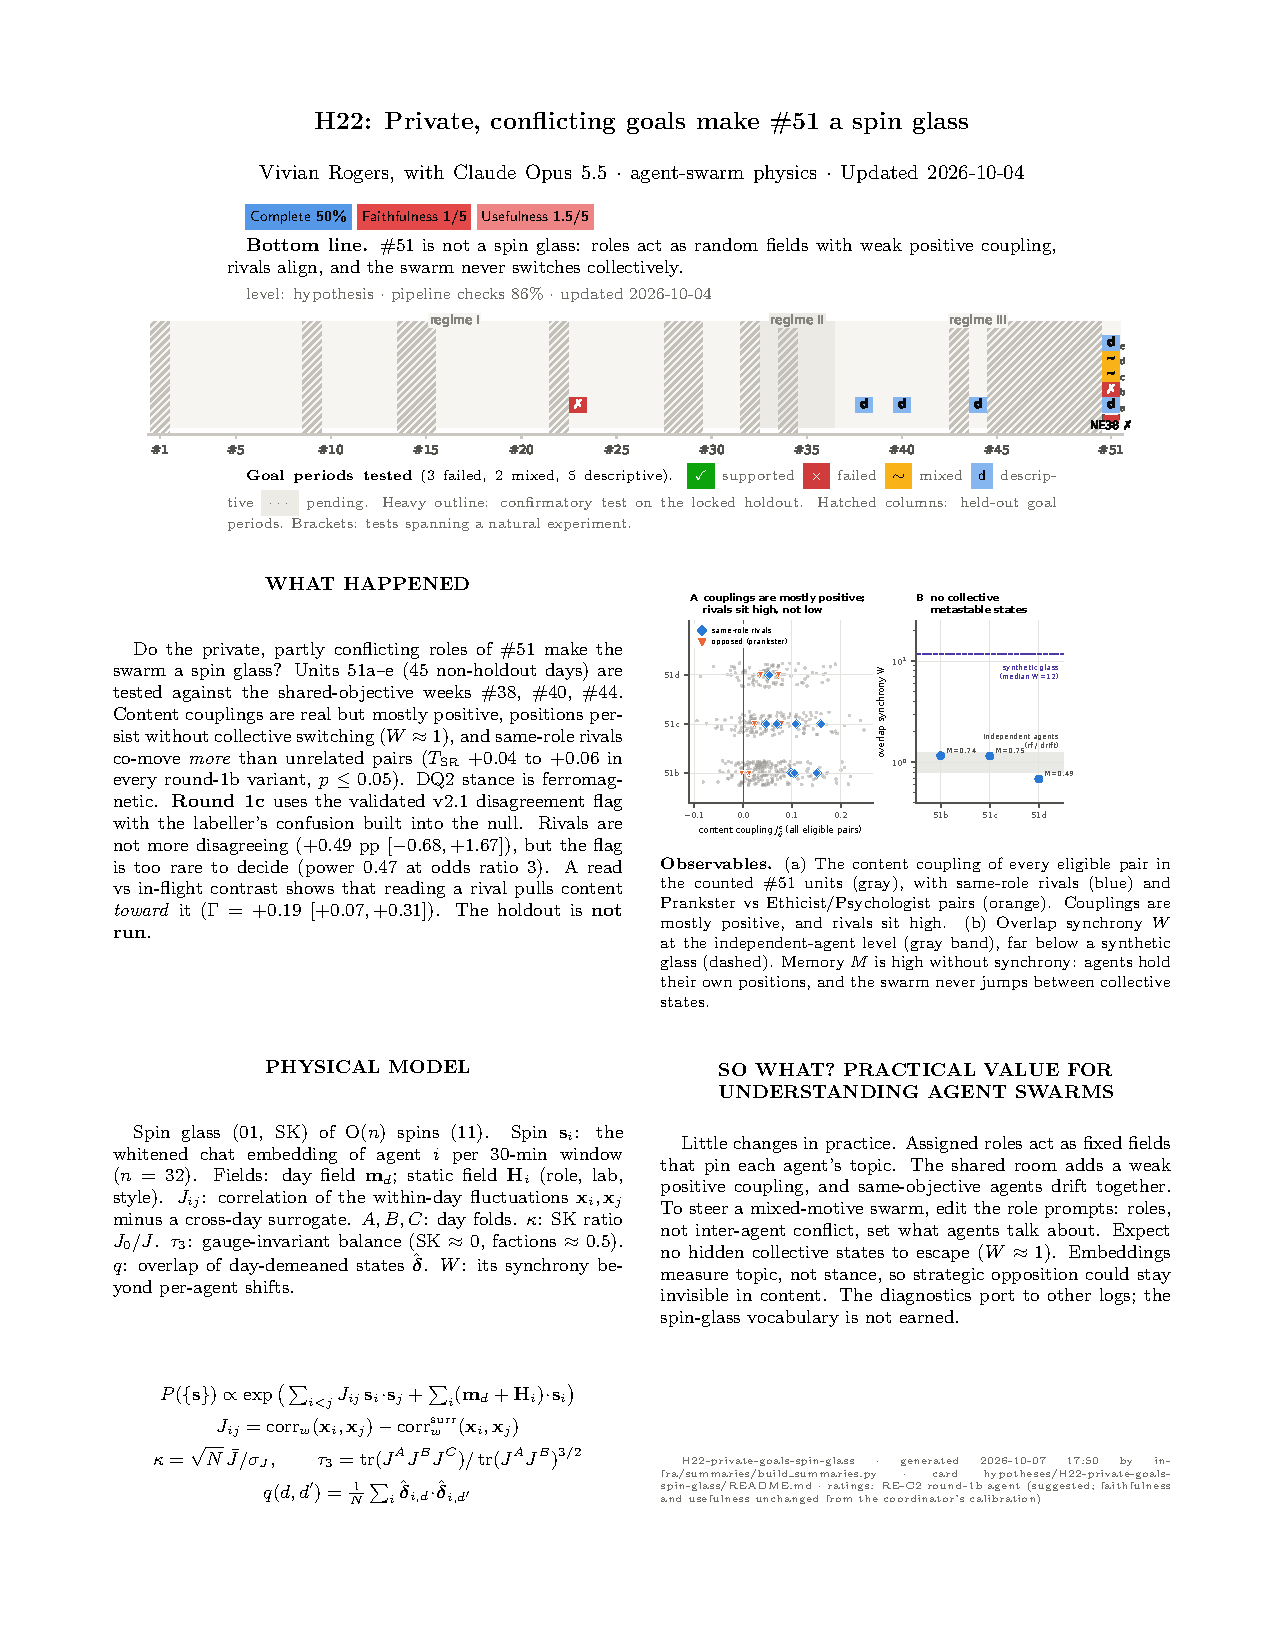
\includepdf[pages=1,link,linkname=H22]{../../hypotheses/H22-private-goals-spin-glass/summary/summary.pdf}
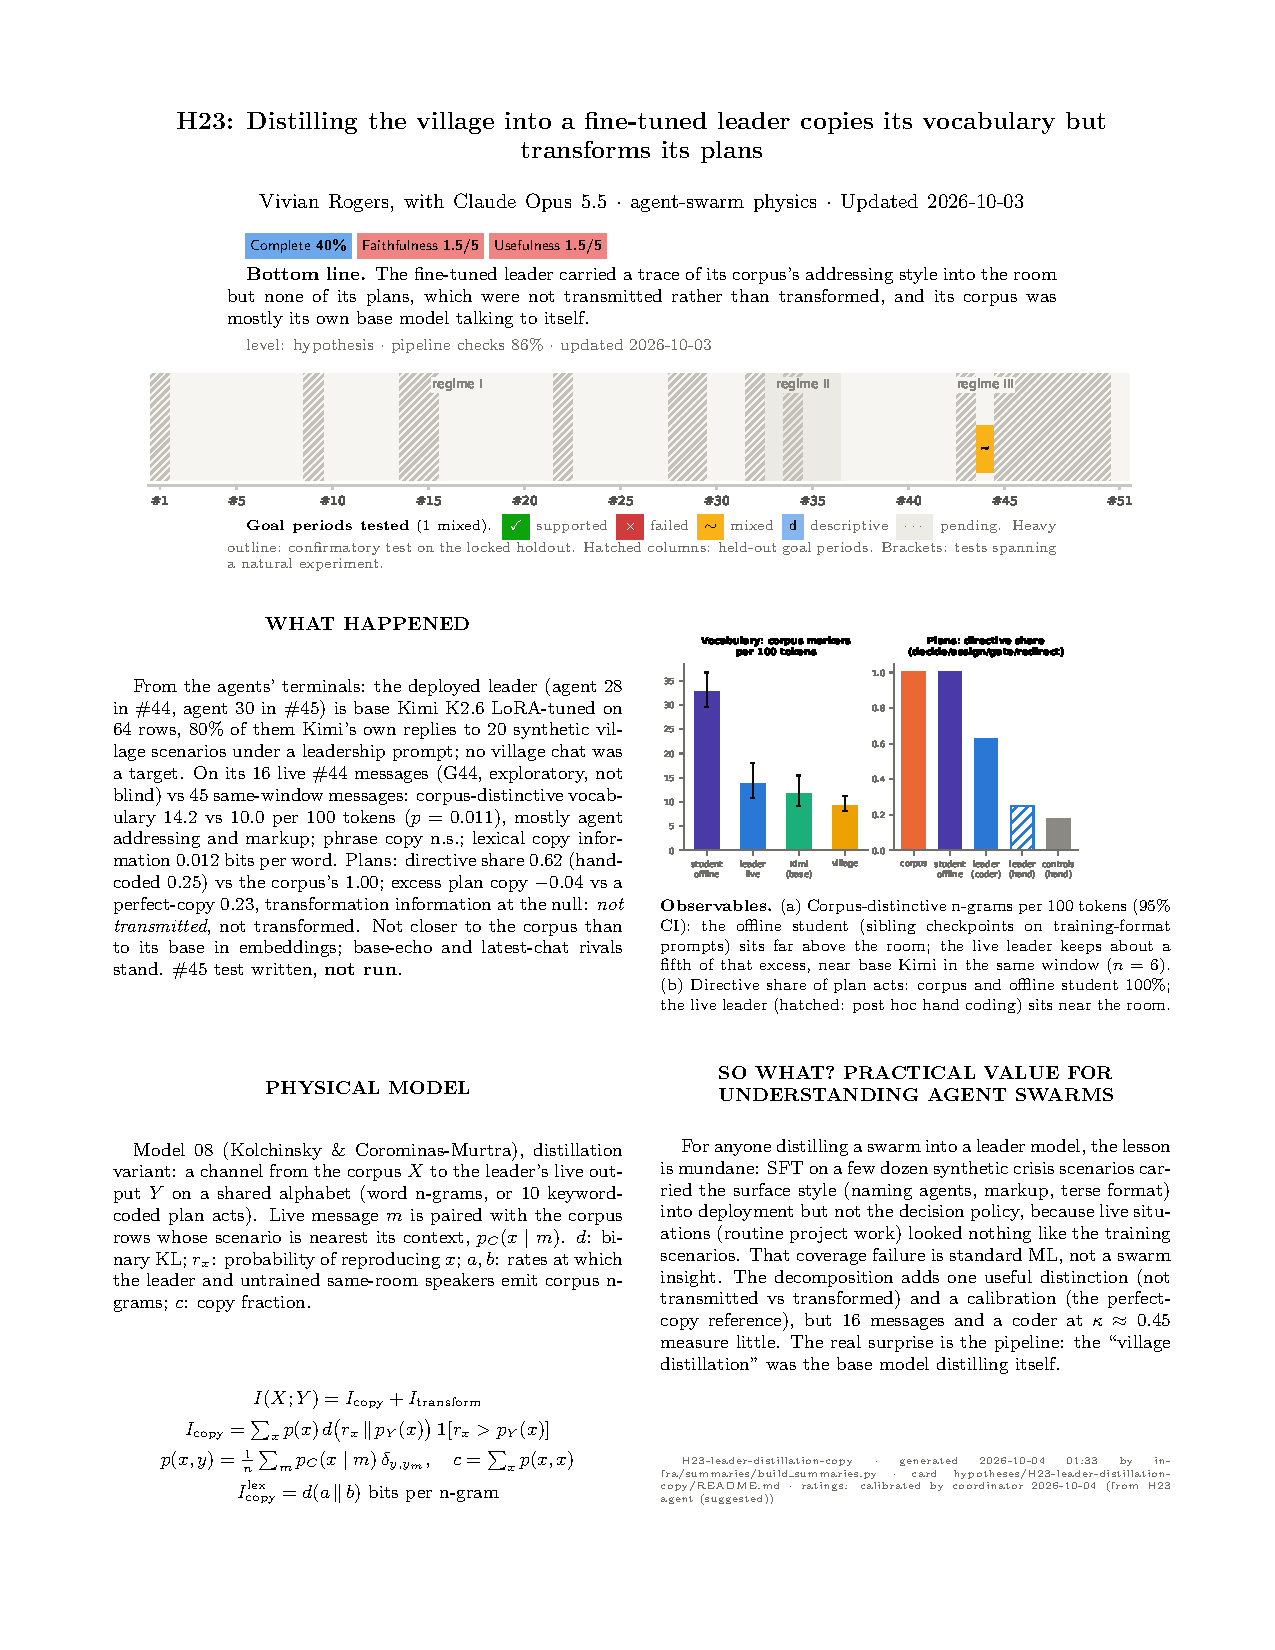
\includepdf[pages=1,link,linkname=H23]{../../hypotheses/H23-leader-distillation-copy/summary/summary.pdf}
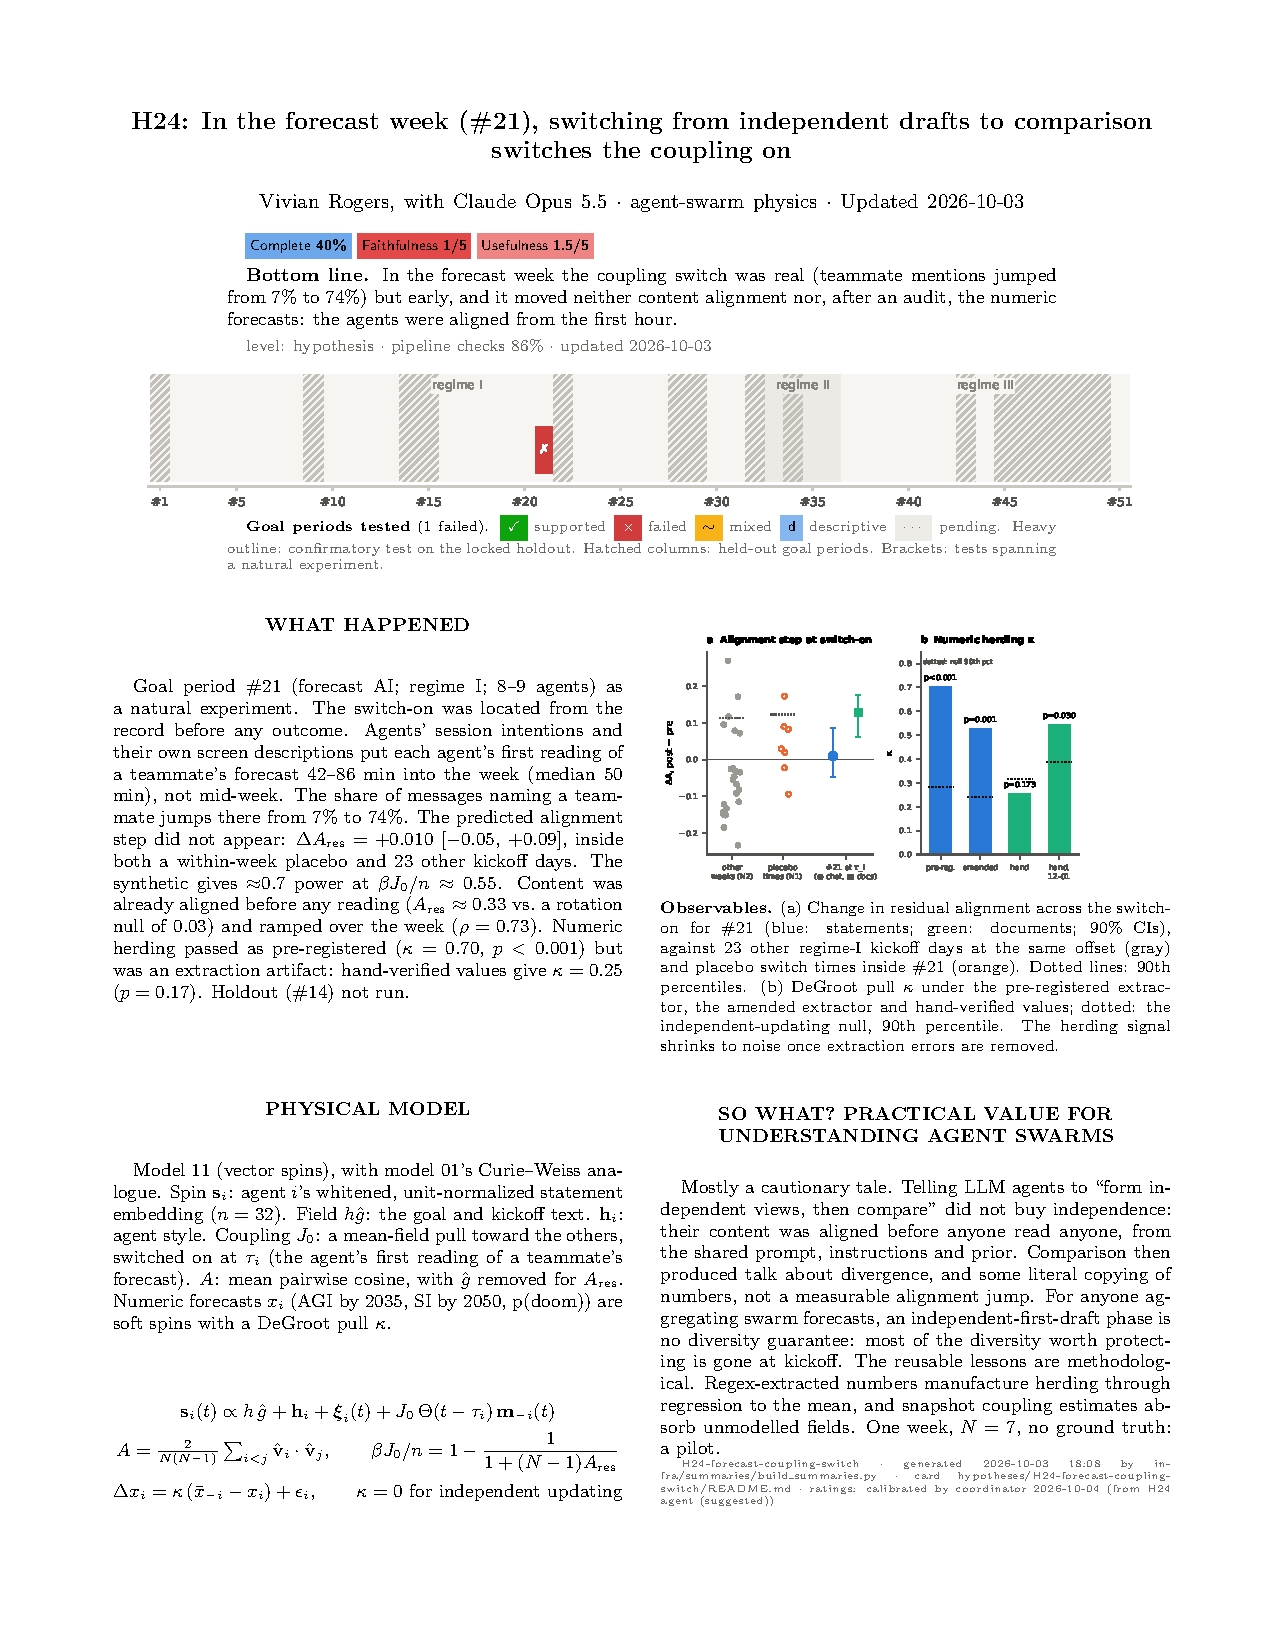
\includepdf[pages=1,link,linkname=H24]{../../hypotheses/H24-forecast-coupling-switch/summary/summary.pdf}
\end{document}
